\chapter{Spatial Estimation In Augmented Reality Aided X-Ray Vision} \label{Chap:X-ray Implemntion}

This chapter explores the parts of \gls{X-ray Vision} that are functional or essential to providing the illusion of looking through an object with the aim of understanding how the visualization can support improved spatial estimation accuracy.
While limiting it's self of OSTAR devices, and utilizing techniques from prior research on other devices this research is able to draw knowledge from some of the most cited \glspl{X-ray Visualization} from \autoref{sec:BackXRayVision} and looks at how users experience placing virtual objects behind or inside a physical world object.
The study presented in this chapter aims to understand the depth and spatial perception challenges and their spatial relationships when using \gls{ost} \gls{ar} \gls{X-ray Vision} by utilizing a method to migrate video footage over and recalibrate it to their real world vision.
Using the findings from this research informs the \glspl{X-ray Visualization} that should be made for \gls{dvr} using \gls{ost} \gls{ar} presented in \autoref{Chap:VolumetricX-rayVision}.

% These results will be evaluated by asking a user to recreate a physical scene within an occluded space using \glspl{X-ray Visualization}.
% This is different to previous works in the space because participants allow users to move around almost freely encouraging participants to use the visualizations in a natural manner.
% This allowed participants to utaize individual strategies and showcasing strengths and weaknesses of the \glspl{X-ray Visualization} regardless of how the user interacted with it. 

Overlaying three-dimensional virtual content on the physical world can be problematic in terms of aligning the perceived depth of the virtual and physical information in AR. 
This is due to AR devices' limitations to present data to people intuitively, and misalignment between the physical and virtual world will present this information as being further away~\cite{Fischer2020a}. 
This is made worse when virtual objects are placed beyond the physical object's bounds~\cite{Bajura1992} as the user's sense of depth is influenced by their ability to recognize visual relationships. When visual cues in AR are not carefully designed, the user may perceive virtual objects to be smaller instead of further away~\cite{Berning2014a}. 
X-ray vision is one approach explored to address some of the challenges of correctly perceiving where virtual objects are positioned in the physical world.

\glspl{X-ray Visualization} have utilized a form of visual saliency~\cite{Kalkofen2007, Sandor2010, Zollmann2010, Kalkofen2013} that was possible by using a \gls{vst} \gls{ar} display that would render the world again from the perspective of a camera.
\gls{ost} devices make this difficult since the user can dynamically see the world through the display. The system does not have a strong picture of the visual saliency the users are looking at. 
This is challenging as there are many different shapes of human heads with eyes placed at different positions; the position that visual objects appear in using an \gls{ost} \gls{ar} \gls{hmd} is it little better than a guess. 
Little focus is on research merging physical and virtual objects with \gls{ost} \gls{ar}, considering depth has been explored.

To make a system more accessible, a system was designed that took \gls{ost} \gls{ar} sensor calibration pipeline that can translate camera footage to a person's sight. 
\gls{ost} \gls{ar} \glspl{X-ray Visualization} benefit from better adapting to changes in the real world and adjusting the visualization to suit what the user is perceiving and is helpful outside of \gls{X-ray Vision} as it allows creation of visualizations or to make virtual objects react to actual world virtual stimuli that any computer vision technology can create.
\gls{ost} \gls{ar} is necessary for several tasks that require the user's vision to be unobstructed, like driving\cite{Gabbard2014}, Surgery\cite{Rolland2000}, and Security operations\cite{Phillips2020} where VST AR HMDs are not suited. \gls{vst} technologies suffer latency issues and are vulnerable to hardware failure, which could be catastrophic for mission-critical tasks like surgery.
\gls{ost} does not suffer from these limitations and may be better suited to the applied tasks above, motivating to investigate further the use of \gls{X-ray Vision} techniques on \gls{ost} technologies.
To adapt \gls{vst} \gls{ar} \glspl{X-ray Visualization}, this research had to overcome several challenges, such as representing the visualization within the correct depth of field and in the appropriate shape the user perceives it to be, which will be explained in depth in this Chapter.


\section{Updates Since Running This Study}

% Gruenefeld et al.~\cite{Gruenefeld2020} performed depth perception studies using an OST headset utilizing x-ray vision, including Grid and Cut-out effects. 
% The grid effect, placed on the ground and a perpendicular wall, could be used to approximate a relationship between the wall and the object. In contrast, the cut-out visualization provided a hole in the wall, which the user could look through to see where the object was on the other side.
% Against a baseline that pointed participants to the object with a red arrow and displayed a perpendicular line going from the far point of the arrow to the bottom of the visualization. 
% Gruenefeld et al.'s~\cite{Gruenefeld2020} found that the weakest of the depth cues were the wireframe and the cut-out. This was because neither of these cues conveyed clear depth indications to the user~\cite{Gruenefeld2020}.

% Another set of studies published by Martin-Gomez et al.~\cite{MartinGomez2021} studied the difference between several \glspl{X-ray Visualization} (None (Superimposition), virtual hole, ghosting, and Random Dot) on both VST AR and OST AR devices in the near field. 
% They found that users better-used \gls{X-ray Vision} on a VST AR headset than on an OST AR device.
% This prompted another study investigating different rendering techniques for \gls{X-ray Vision} (shading, hatching, ghosting) and brightness levels, finding that bright, clear objects work best in OST AR.

Since running this study, several similar studies have published their results as are detailed in \autoref{sec:ComparisionOfDisplays}. 
This research maintained its novelty by evaluating the effects of various VST AR effects, such as Saliency and Edge-Based techniques.
These techniques have not been compared against \textit{Random Dot} and wire-frame \glspl{X-ray Visualization}.
Moreover, previous studies commonly restricted the user's movement while investigating the different approaches to depth cues. 
Rather, This work focuses on a more natural interaction with these effects, looking at a less restrictive solution to test the uses of various \glspl{X-ray Visualization} to understand better users' natural processes for dealing with different types of occlusion.


\section{Adopting X-ray Visualizations for Augmented Reality} \label{sec:X-ray Vis}

% paragraph explaining 
% why,
% partial occlusion
% 
This research chose to focus on auxiliary effects (using groups of objects) and \glspl{X-ray Visualization}. 
many medical applications will likely cause some auxiliary effects in the data, because most medical applications will require the user to look through a large amount of data to find a small part of interest. 
Auxiliary effects work by introducing additional reference objects or visual cues into the scene, helping users to better judge spatial relationships and depth.
In the context of volume rendering, auxiliary effects can include the placement of markers, or anatomical landmarks within or around the volume. 
These added elements provide extra context, making it easier for users to locate, interpret, and interact with regions of interest within complex volumetric data. 
By enriching the visualization with supplementary information, auxiliary effects help users navigate dense or ambiguous data, reduce cognitive load, and enhance overall spatial understanding.

The \glspl{X-ray Visualization}s chosen for this study were:
\begin{enumerate}
    \item Edge and Saliency techniques occluded large amounts of the data behind the objects, while the other two drew lines over the object you were trying to look through. Creating a High Occlusion Model and a Low Occlusion Model for dynamic effects.
    \item The other consideration was using geometric saliency vs. visual saliency (or Real-world Overlays vs. Computer Vision Enabled \gls{X-ray Vision} techniques). Since there is no record of using Computer Vision Enabled \gls{X-ray Vision} techniques on stereoscopic \gls{ar} devices.
\end{enumerate}
Hole-in-the-world visualizations were ruled out as limiting the view of the visualization, requiring more volume data to be produced. Four visualizations were chosen due to the differences in their designs.
Instead, a back face to this was applied to the cube, which has been shown to improve depth perception~\cite{Lerotic2007}.

Four types of \gls{X-ray Visualization} techniques are utilized for use with \gls{ost} \gls{ar} displays: \textit{Random Dot}, \textit{Tessellation} (similar to wireframe), \textit{Edge-Based}, and \textit{Saliency}.
These visualizations were chosen because they were all only utilized up to this point for \gls{vst} \gls{ar} \gls{X-ray Vision} Papers.
\textit{Edge} and \textit{Saliency} used Computer Vision-Enabled Techniques, while the other two utilized a Real-world overlay (\textit{Random-Dot} and \textit{Wireframe}). This could then further be split as one from each of these groups blocked out a large portion of the user's vision (\textit{Random Dot} and \textit{Saliency}), while the other used thin lines to show contrast to the world via the display (\textit{Edge} and \textit{Wireframe}).

% Placed here to help with the flow of  content should logically be lower
\begin{figure}[tb]
    \centering
    \includegraphics[width = \textwidth]{Chapter3/Images/Visualizations/OtsukiRandomDot.png}
    \caption[a) Otuski et al.'s~\cite{Otsuki2015} version Random Dot b) A image of the \textit{Random Dot} visualization used in this chapter.]{a) Otuski et al.'s~\cite{Otsuki2015} version Random Dot b) A image of the \textit{Random Dot} visualization used in this chapter. Taken using a HoloLens2 under study conditions. a) Was produced by By Otuski et al.~\cite{Otsuki2015} and is licensed under a Creative Commons Attribution licence}
    \label{fig:RandomDotImage}
\end{figure}

Any virtual object that is partially occluded by another virtual object is in front of a given object~\cite{Bajura1992, Vishton1995}. 
However, to make this a seamless experience, it is required to experience this.
Research on all these techniques has shown the importance of partial occlusion, but no work has been done comparing their ego-centric constraints to this point~\cite{Sandor2010, Dey2012, Dey2014, Zollmann2014, Tsuda2005}.
While other studies have researched the impact of the amount of occlusion, these forms of \gls{X-ray Vision} can bring~\cite{Santos2016}, which have been used and considered when designing the parameters used when adapting these visualizations.
However, all these studies were much more controlled than ours and were run using a range of \gls{vst} devices. 

Regardless, some of the technical considerations for each of these visualizations have been adapted around the same environmental considerations to ensure the visualizations are as fair as possible.
Firstly every visualization utilized a back face to the cube, because it has been shown to improve depth perception~\cite{Lerotic2007}.
The back face was a contrasting pink color that contrasted with the virtual objects and the large Voronoi cube (shown in \autoref{fig:Basic image of setup}).
Placing a plane on any face of the cube that is facing away from the user that is visible in AR. 
Once a virtual object goes past the back face, it will begin to clip behind this object until it is no longer visible to the user.

The X-rayable area was the 0.6m x 0.6m x 0.6m area within the cube between the backface of the effect and all the \glspl{X-ray Visualization} except for the baseline No \gls{X-ray Visualization} (referred to as \textit{None}).
\textit{None}  which provided no occlusion over any part of the virtual objects within the x-rayable space. 
Simply, it superimposes the visualization of the objects.
To the user \textit{None} would likely appear to the user to seem as if the back plate of the X-rayable area was in front of the x-rayable area even though it is technically in the same area for each condition.

\subsection{Random Dot X-ray Visualization}

\textit{Random Dot} appears as a grid of square dots that can be turned on or off. 
Generally, these are colored a slightly translucent shade of black \autoref{fig:RandomDotImage}. 
The instance of \textit{Random Dot} used in this study uses the translucent shade of white \autoref{fig:RandomDotImage} b, since \gls{ost} \gls{ar} headsets can not render black.
Random Dot was a \textit{real world overlay \gls{X-ray Vision} technique} was used because it relied on \gls{slam}~\cite{Karlsson2005, Klein2007} for positioning and obscured some of the user's vision into the X-rayable space and geometrical saliency, akin to \textit{Saliency}. 
The implementation of this visualization followed the published description of the visualization by Otsuki et al.~\cite{Otsuki2016, Otsuki2017}, with a scale for different-sized dots and density, 
a low-resolution texture (50 x 75 px), and randomly made half of the pixels either transparent white or clear.
%This resolution was chosen because it  best fits our real-world environment.

\begin{figure}
    \centering
    \includegraphics[width=\textwidth]{Chapter3/Images/Visualizations/livingstoneWireframe.png}
    \caption[a) Livingston et al.'s~\cite{Livingston2003} initial version of the wireframe \gls{X-ray Vision} effect b) A image of the \textit{Tessellation} visualization used in this chapter.]{a) Livingston et al.'s~\cite{Livingston2003} initial version of the wireframe \gls{X-ray Vision} effect b) A image of the \textit{Tessellation} visualization used in this chapter. Taken using a HoloLens2 under study conditions. a) Was used with permission from IEEE \textcopyright{} 2003}
    \label{fig:TesselationImage}
\end{figure}

\subsection{Tessellation X-ray Visualization}

Wireframes have long been used as \glspl{X-ray Visualization}, giving the user some identification of where the real world is compared to the virtual world and being able to provide some identification of minor occlusion~\cite{Tsuda2005, Webster1996}.
%The \textit{Tessellation} visualization shown in \autoref{fig:TesselationImage} shows a similar but different take on the same properties as a wireframe model was chosen over a wireframe visualization to allow for flexibility~\cite{Hettinga2018} by allowing geometrically salient patterns without needing to add any extra polygons.
The \textit{Tessellation} visualization shown in \autoref{fig:TesselationImage} shows a similar but different take on the same properties as a wireframe visualization but is using a geometry shader and calculating a uniform dimension for each of the tiles to become between each edge of the shape. 
This allowed for flexibility~\cite{Hettinga2018} by allowing geometrically salient patterns without needing to add any extra polygons.

\textit{Tessellation} subdivides a wireframe into more triangles, covering more area. 
Generally, this is done to increase the quality of a virtual object by creating increasing the polygon count without adding extra geometry~\cite{Hettinga2018}, but in this case, it was used to create a wireframe-like effect that could be adjusted to cover more or less of the cube.
This visualization subdivided an existing wireframe further and would normally be designed to allow for a dynamic range of quality to be applied to a virtual object~\cite{Hettinga2018}.

A uniform Tessellation algorithm was used to ensure the triangles were placed in an even and logical manner. 
The uniform triangular tessellation using fractional-odd partitioning on triangle patches where each original triangle gets subdivided into smaller triangles. This was set to produce five regular and evenly distributed across the entire surface~\cite{flick_2017}.
Allowing complete flexibility to manually manipulate the size of the effect to choose the amount of the cube covered by the effect.
For this application, a uniform \textit{Tessellation} was utilized to keep the quality increased amount and aimed to create five new lines coming out of each edge~\cite{flick_2017}. %This is technically where I got the idea for this effect
This allowed a visualization seen in \autoref{fig:TesselationImage} like a Wireframe and retained geographical sense while maintaining realistic and continuous while also manipulating the total number of lines, allowing for more partial occlusion. 

\subsection{Edge-based}

The \textit{Edge-Based} visualization places a white line over all areas that show contrast between sets of neighbouring pixels. 
This visualization was selected, since as seen in \autoref{fig:edgeBasedImage}, the \textit{Edge-Based} visualization occludes very little of the user’s vision and uses salient points of interest in the user's own point of view to provide the visualization.
Designed initially by Kalkofen et al.~\cite{Kalkofen2007}, this visualization provides just enough occlusion to show virtual objects as opposed to the visually salient parts of real-world objects, effectively guiding users to discern the presence and location of virtual entities.
The Sobel algorithm was utilized for this implementation with a delta X and delta Y of 5 (performing the algorithm over a 5 by 5 grid).
The Sobel algorithm was chosen over other edge-based detection algorithms due to how well it performed in parallel, using only a single step, unlike other edge detection algorithms, such as the canny edge detection. 

\begin{figure}[tb]
    \centering
    \includegraphics[width=\textwidth]{Chapter3/Images/Visualizations/KalkofenSaliency.png}
    \caption[a) Kalkofen et al.'s~\cite{Kalkofen2007} version of \gls{X-ray Vision} b) A image of the \textit{Edge-Based} Visualization used in this study.]{a)Kalkofen et al.'s~\cite{Kalkofen2007} version of \gls{X-ray Vision} b)A image of the \textit{Edge-Based} Visualization used in this study. Taken using a HoloLens2 under study conditions. a) Was produced by Kalkofen et al.'s~\cite{Kalkofen2007} and was used with permission from IEEE \textcopyright{} 2007}
    \label{fig:edgeBasedImage}
\end{figure}

\subsection{Saliency}

Visual saliency describes how much a given object or region in a scene may stand out or attract attention to the viewer. 
As mentioned in previous chapters, Sandor et al.~\cite{Sandor2010} found that by using by showing attention-grabbing objects in the foreground, you could create an \gls{X-ray Vision} visualization that communicates to users with a good level of depth perception where an object exists. 
\textit{Saliency} was chosen for this study because it partially occludes some of the user's vision, like \textit{Random Dot}, and uses the visually salient regions in the user's own point of view, similar to the ~\textit{Edge-based} visualization.
Tian et al.'s~\cite{Tian2009} Saliency algorithm was adapted to run in parallel on a GPU.
This first required the HSL (Hue Saturation and Intensity) value~\cite{Valensi1945} to be extracted from the RGB color using a similar method to Saravanan et al.~\cite{Saravanan2016}.
The values of the individual Hue, Saturation, and Intensity Contrast were then calculated along with the Dominance of both the warm colors and the Saturation and Intensity.
These methods were then normalized and weighted by utilizing a static set of values that were calculated prior based on the lighting of the study environment. 
The study environment provided consistent lighting and colors to ensure these values remained consistent.

Unlike the other visualizations, the \textit{Saliency} algorithm would utilize salient features from the real world to occlude the virtual objects~\cite{Sandor2010}.
VST AR devices normally do this by rendering the real world partially on top of the virtual world. 
%This will not work in using \gls{ost} \gls{ar} as the real world is not rendered using a stereoscopic video feed, it is a person's actual vision. 
In VST AR, depth is reconstructed from a stereoscopic camera feed, but in OST AR the user sees the real world directly through transparent optics.
Making it difficult to know what the user is looking at and how to occlude the virtual objects over users vision of the real world. 
To get around this issue, the visualization used in \autoref{fig:saliencyImage} was used. 
Instead of producing saliency over the top of real-world constraints, this version of saliency would make more salient areas of real-world objects more opaque and others less opaque by rendering a black area over the x-rayable area. 
Rendering the salient areas as black enabled the system to interpolate between fully occluding the object and being completely transparent without the user being able to view these abilities. 

\begin{figure}[tb]
    \centering
    \includegraphics[width=\textwidth]{Chapter3/Images/Visualizations/SandorSaliency.png}
    \caption[Two images that use saliency detection. a) Sandor et al.'s~\cite{Sandor2010} version of Saliency. b) An image of the \textit{Saliency} Visualization used in this study]
    {
        Two images that use image saliency detection to find area's of human interest within the images to occlude virtual objects.
        a) Sandor et al.'s~\cite{Sandor2010} version of Saliency which changes the opacity of objects in the foreground to reveal another video image in the background. b) An image of the \textit{Saliency} Visualization used in this study which increases the occlusion of the real world objects by creating a transparent mask over the top of the objects from drawing back in the screen a color that the HoloLens is unable to display at varying angles. b) Was taken using a HoloLens2 under study conditions.
        In this setup, the large cube was decorated with a Voronoi pattern of brightly coloured tiles.
        These coloured tiles acted as salient features: the irregular edges, strong contrasts, and varied hues provided multiple points of visual interest that the saliency algorithm could reliably identify. This ensured consistent saliency detection across the cube’s surface, while also preventing participants from relying on simple geometric cues such as uniform grids.
        a) Was produced by Sandor et al.'s~\cite{Sandor2010} and was used with permission from IEEE \textcopyright{} 2010
    }
    \label{fig:saliencyImage}
\end{figure}

%, so they would suit the study environment better. 
% The rectangular shape of the dots was chosen due to the user’s general orientation to the cube. 
%No immersive OST AR applications have ever overlaid a picture of the real world 
\textit{Edge-Based} and \textit{Saliency} \glspl{X-ray Visualization} required major additions to their calibration to make them work with OST AR devices are described in detail in the next section (\autoref{sec:X-ray VST Overlay}).

\section{Rendering Considerations} \label{sec:X-ray VST Overlay}
To take advantage of \glspl{X-ray Visualization} that were traditionally designed for VST AR systems, A system that could transmit camera data over to an OST AR display was required. 
%This would allow the system to highlight areas of high visual impact. 
The following system was designed to display the output of a video feed over a user's vision for x-ray vision, allowing the system to highlight areas of interest in the user's vision. However, its potential uses are not limited to this.

\subsection{Video Image Overlay Method} \label{sec:X-ray VST Overlay Method}
% What is the problem that this area is addressing
Calibrating video see-through techniques, such as \textit{Saliency} or \textit{Edge-Based} visualizations for see-through video headsets and mobile devices~\cite{Avery2009, Sandor2010}, presents the need for a change in calibration as a 2D image will need to be able to respond to the user's depth cues to present the correct affect~\cite{Li2012}. 
This system would need to accommodate the difference between the distortion of human sight~\cite{Peek2014}, reacting to their movements as fast as possible~\cite{Wang2023, Li2012} while understanding the depth of field.
To date, no algorithms for \textit{Saliency} or \textit{Edge-Based} visualizations were found that made use of bifocal vision\cite{Otsuki2016, Otsuki2017}, with each eye requiring its display that would not overlay onto a video feed but the participants’ view of the real world. 
The closest method previously used was Hamadouch's~\cite {Hamadouche2018} method, which displayed \textit{Edge-Based} \gls{X-ray Vision} using projectors in collaboration with the HoloLens2. 
Our technique extended this concept by applying \gls{X-ray Vision} visualization to a virtual projector, creating the illusion of depth within the augmented world and aligning the virtual objects with the view of the physical world through the headset. 

% Explaining at a high level what the distortion was doing
As illustrated by \autoref{fig:FrameByFrameGuide}, each time a new image from the video feed was received, the image was filtered to represent either a \textit{Saliency} or \textit{Edge-Based} map and then distorted to align with the users' vision. 
This image was then used as input into a virtual projector from the user's perspective but only interacting with the X-rayable object.
Outputting either a color-based saliency map for the \textit{Saliency} condition or a Sobel edge detection for the \textit{Edge-Based} visualization, 
This was then distorted for each of the user's eyes. 
For \textit{Saliency}, a shadow occludes the graphics rendered within the cube, while a white light was projected for an \textit{Edge-Based} visualization.

\begin{figure}
    \centering
    %\includegraphics[width=\columnwidth]{Chapter3/Images/ViewPerspectivesBetter.png}
    \includegraphics[width=\columnwidth]{Chapter3/Images/ViewPerspectivesBetterNoDepthPlane (1).png}
    \caption[This image illustrates how different fields of view (FOV) were managed to work with each other.]{This image illustrates how different fields of view (FOV) were managed to work with each other. 
    The yellow line indicates the user's entire bifocal field of view ($130^\circ$ vertically).
    The red lines show the Field of View (FOV) of the HoloLens2 from the user's point of view ($29^\circ$ vertically).
    The blue lines show the FOV of the ZED Mini from the position it was mounted ($54^\circ$ vertically).}
    \label{fig:ViewPerspectives}
\end{figure}

The HoloLens2 was used as the OST AR device, and a ZED Mini stereo camera~\footnote{\url{https://www.stereolabs.com/en-au/store/products/zed-mini}} was used to capture the video feed.
The ZED Mini was chosen due to its small size, stereoscopic video feed however this this use the inbuilt funciationlity of the was not required as the hovermap was able to provide this and the distortion algorithm is incorrect for this use case.
The ZED Mini was mounted on the front of the HoloLens2, as close to the user's eyes as possible, as shown in \autoref{fig:ViewPerspectives} using a custom 3D printed mount described in \autoref{sec:X-rayAddionalSensors}.


% Explaining how the initial offset was fixed
On an OST AR display, it is impossible to mount a camera that will see the world from the same perspective as the user, so these cameras need to be placed away from the user's view. 
First, the offset needs to be applied to the virtual world to overlay the image from the camera.
% Talking about the radial distortion
Radial distortion is required to match the virtual representation of the real world so that the virtual content the camera produced is accurately aligned with the user's vision~\cite{Brown1966, Zhang1998, DeVilliers2008}. 
By applying this to the visualization frame, the edges of the display were matched to the user’s vision of the real world. 
Since the eye movements of the user required some input from their bifocal cues, the distance-based distortion algorithm~\ref{alg:distortionAlgorithm}) was applied to the visualization from the headset. 
This required the distance from the user and the visualization to be tracked, as the difference in perspective between the camera and the headset would need to be compensated for. 
Influencing the value along the input camera image's vertical axis (height position).
Linear interpolation was used to estimate any unrecorded values between the known ones.
This gave the user the impression that the projection was aligned appropriately on the box.

The used parameters used to correct the distortion and the perspective offset calculated from the participants subjective feedback during a short test after the pilot study.
Each of the participants used in the pilot study was asked to view the visualizations overlaid on the box from 3 different distances (0.5m, 1m, and 1.5m) at three different orientations on the box with the request provide feedback on the alignment of the visualization.
This feedback was used to adjust the distortion values for the given depth away from the camera was positioned repairing the offset between the camera and the HoloLens display as well as translating the image distortion to from the camera to match the user's vision.

\begin{algorithm}
    \caption[Algorithm for the radial distortion used by the camera.]{Algorithm for the radial distortion used by the camera. This is a standard GPU variant of the Radial Distortion Algorithm~\cite{Kang2001, Liu2025, Brown1971}. All variable values are Vector2s, except for D, which is the distortion value and indicates the level of distortion required at a given pixel. To correctly distort the image to resemble human sight, outlet areas of the viewing area, depending on the viewpoint of the user, will need to use barrel distortion, while other inner areas will use pincushion distortion.}
    \label{alg:distortionAlgorithm}
    \begin{algorithmic}[1]
        \State $uv \gets (uv - 0.5) \times (D_z + 0.5)$
        \State $ruv \gets {DScale_x}_y \times (uv - 0.5 - {DCenter_x}_y)$
        \State $ru \gets \text{length}(ruv)$
        
        \If{$Pincushion\_Distortion$} 
        \State $uv \gets uv + ruv \times ((\tan(ru \times D_x) \times (1.0 / (ru \times D_y))) - 1.0)$
        \Else 
        \State $uv \gets uv + ruv \times (((1.0 / ru) \times D_x \times \arctan(ru \times D_y))) - 1.0)$
        \EndIf
        \State $return \gets uv$
    \end{algorithmic}
\end{algorithm}

In order to make the visualization appear as if it were being projected from the user's perspective, the system needed to understand where the user was looking and how far away they were from the box however since the pipeline took approximately 50ms to reach the display it was important that the system could predict the closest point the user would have been looking at when the image was taken.
to accomplish this the camera output is then rendered based on the location where the image was taken, invisible to the user for the first frame until it is projected on the next frame in the same place the image was taken.
This allows the user to see the image from the camera as if it were being projected from the user's perspective.
\autoref{fig:ViewPerspectives} illustrates that the Camera had a wider field of view than the HoloLens2, so the user could move around within the FOV of the camera without losing the visualization.
One issue to this methodology is that the field of view of the \gls{X-ray Visualization} is limited to interactions that are approximately within 10 cm from the box past this point the visualization will be cut off by the edge of the camera's field of view.

\begin{figure}
    \centering
    \includegraphics[width=\columnwidth]{Chapter3/Images/FrameByFrameGuide.png}
    \caption[This diagram explains the frame-by-frame process that the system used to process images]{This diagram explains the frame-by-frame process that the system used to process images; each frame away from receiving the first images is labeled up the top of the diagram. Each system task is listed in a square box. ZED Mini describes the process where the ZED Mini provides the system with the image. Filter explains whether the Sobel edge-based filters are applied. The render state is when the final scene is distorted and rendered to be overlaid onto the user's vision.}
    \label{fig:FrameByFrameGuide}
\end{figure}

% I'm thinking about drawing a diagram of this
The \gls{ost} \gls{ar} \gls{hmd} used for this experiment (a HoloLens2) required a tethered connection to receive a video feed from the camera as initial testing from the inbuilt camera showed several issues: The battery life of the devices decreased dramatically. The performance of the system dropped to a maximum frame rate of 30\gls{fps}; the image had a low quality, and it had been extensively processed. 
A tethered connection would inevitably cause a delay in when the system would need to be known.

The delay between the camera to the computational server and the display was tested using a system similar to Gruen et al.'s\cite{Gruen2020} system and found the camera (the ZED mini) produced a video lag of approximately 50ms from when the image was captured to being displayed by the OST AR Headset (HoloLens2). 
The lag is noticeable when viewing within an OST AR headset. 
To overcome this, a 5 Gbit/s USB connection between the OST AR Headset and the PC was used to render the visualization, enabling a rapid and stable visualization between the system and the OST AR Headset.
Most of the lag occurred between when the picture was taken and when the system could process it.

To compensate for this lag, the asynchronous re-projection algorithm was implemented, which recorded the position the user was looking at each frame using the manner seen in \autoref{fig:FrameByFrameGuide}, and used the position recorded three frames before the picture was acquired in the systems calculations~\cite{VanWaveren2016,  Landvoigt2017}. 
This approach enabled the system to place the image at the approximate position it was taken since the re-projection accounted for ~48ms (3 frames) of the delay.

% talking about how the noise reduction was managed
This system also introduced noise created from a) the difference between the estimated and actual positions of where the picture was taken and b) the user's involuntary head movements (e.g., \Gls{microsaccades}~\cite{Martinez-Conde2013}). 
To repair the damage done by the difference between the estimated and actual positions, the position and orientation where each image frame should have been were rendered, and the image was distorted to match that position. 
%calculate where each image frame would have been rendered. 
The system would then render the frame it received at the position where the user was looking four frames ago.
This would give the system a frame to apply the Sobel or saliency filter and apply the distortion mentioned earlier.

% talking about how the output was smoothed
To help with the \gls{microsaccades}, the position of the output image was first sent into a one euro filter~\cite{Casiez2012}. 
The filter provided the flexibility to allow large sweeping head movements to appear as if they had no latency but filtered values when the user stopped moving. 
This kept the image where the participant expected it without restricting their movement. 

% Explaining the preliminary study that was used to determine the exact parameters
A preliminary study of 5 participants was used to determine the correct parameters for the filter. 
Each participant used the system for 5 to 10 minutes and was able to set the parameters. 
This resulted in the following parameters being selected:
One euro filter’s frequency was set to 60, with a min cut-off set to 1, the beta was set to 200, and the D cut-off was set to 1.
These settings would turn off the filter when the user was making large motions like turning but would keep the image stable when they were standing relatively still. 

% The frequency with this system updated the image
The system was sent a new image every frame that corresponded to the position the user was in approximately 50ms prior. 
The \textit{Edge-Based} and \textit{Saliency} visualizations had an approximately 50ms slower start-up time than the wireframe and \textit{Random Dot} visualizations. 
The system ran on the HoloLens with a constant frame rate of 60 frames per second. 
Our system could achieve this consistently across all visualizations, which was consistent with the camera, allowing for a close match to the user's perceived real-world view and the input video feed.

\section{Pilot Study} \label{sec:X-ray Pilot}
%derived our hypotheses based on a preliminary study that was run 
A pilot study was conducted prior to the main study to test the viability of the \glspl{X-ray Visualization} running on an \gls{ost} \gls{ar} \gls{hmd} on a cohort of 5 participants to test depth perception. 
This was done by comparing the participants' performance of a \gls{vst} \gls{ar} \gls{hmd} against their performance using an \gls{ost} \gls{ar} \gls{hmd} to determine if there were any distinct differences between the implementations on a given headset.
Similar to the design of studies done by Otsuki et al.\cite{Otsuki2017} and Martin-Gomez et al.\cite{MartinGomez2021} using the large Voronoi cube (shown in \autoref{fig:Basic image of setup}) where the participants were asked to guess what geometric shapes where inside or outside of the box if they could determine it.

The participant sat in a chair 1.5 meters away from the cube and was required to say if any of the three provided objects (a sphere, a cube, and a star) were inside it.
No object would appear to be partially inside of the cube
The answers they could give were to say if they were certain it was inside the cube, they were certain it was outside the cube, or they were unsure if it was inside or outside the cube. 
These objects were randomly placed either inside or outside of the object.

Both the \gls{vst} and \gls{ost} systems used a ZED mini~\footnote{\url{https://store.stereolabs.com/en-au/products/zed-mini}} to provide the system with visual information.
The \gls{vst} \gls{ar} \gls{hmd} was built from a Vive pro~\footnote{\url{https://www.vive.com/au/}} using a ZED Mini to provide \gls{ar} support.
The \gls{ost} \gls{ar} \gls{hmd} was a HoloLens2~\footnote{\url{https://www.microsoft.com/en-au/HoloLens}} using a ZED Mini as the system's visual input. 

The pilot study was tested using a Friedman test with a post-hoc Wilcoxon signed-rank test with a Bonferroni correction to determine if there were any significant differences between the different visualizations and devices.
The results of the pilot study are to remain confidential due to the ethics agreement; however we did find that Saliency and Random Dot were the most effective visualizations for depth perception.
Regarding the differences between the displays this pilot had similar results to Martin-Gomez et al.'s\cite{MartinGomez2021} test regarding both devices, where both devices produced a significantly different effect in regard to depth-based accuracy, with VST AR being more accurate but having many more uncertain answers.
%No other metric showed a significant difference related to depth. 
%The visualization effect was insignificant; however, 
\textit{Saliency} proved the most effective \gls{X-ray Visualization} for depth perception, with \textit{None} being the worst. 
A System Usability Scale (SUS) showed that people preferred to use the Computer Vision-Enabled Techniques (\autoref{sec:ComputerVisionEnabledTechnqiue}).
Possibly due to the small amount of participants these results showed very few significant differences(p-value $>$ 0.05).

\section{User Study} \label{sec:X-ray User Study}



\begin{figure}
    \centering
    \includegraphics{Chapter3/Images/Visualizations/None.png}
    \caption{A image of the Baseline (\textit{None}) condition}
    \label{fig:BaselineImage}
\end{figure}

A placement task assessed how well participants could place virtual objects within a large physical cube decorated with a colorful Voronoi pattern (shown in \autoref{fig:Basic image of setup} and \autoref{fig:BaselineImage}). Users could walk freely within a prescribed area in the study environment detailed in \autoref{fig:Study One Set up}.
This allowed for a more natural interaction with the virtual objects and the environment and provided a more realistic scenario for how these visualizations would be used in practice than testing depth based alignment tasks.
Allowing movement was essential because depth judgments in AR rely heavily on motion parallax and viewpoint changes, which cannot be experienced in a seated, fixed-position setup. Furthermore, in practical AR applications users naturally move around objects to inspect them from multiple perspectives, so incorporating movement provided both stronger perceptual cues and a more ecologically valid evaluation of the visualization techniques than a purely seated, static study.
In order to ensure that participant specific skills like hand-eye coordination, spatial reasoning, and motor skills did not affect the results of the study, a within-subjects design was used where each participant experienced all conditions of the study, along with a random effects style analysis to control for individual participant bias.

The pilot study described in \autoref{sec:X-ray Pilot} which was used informed the design of this study and to provide a comparison between the two types of \gls{ar} devices.
Since for this Dissertation there was a requirement to use an \gls{ost} \gls{ar} device to enable these visualizations, it was decided that the main study would only use an \gls{ost} \gls{ar} device so the all that was required was to compare the different \gls{X-ray Visualization} techniques.
While alignment tasks or comparisons to \gls{vst} \glspl{hmd} could provide baseline performance measures, they would not isolate the contribution of visualization techniques.
The study therefore focused on comparing alternative visualizations within \gls{ost} \gls{ar}, as this directly addressed the research question of how X-ray visualizations perform in see-through displays.


Participants were either assisted with one of the four \gls{X-ray Visualization} techniques \textit{Random Dot} (\autoref{fig:RandomDotImage}), \textit{Tessellation}, \textit{Edge-Based} (\autoref{fig:edgeBasedImage}), and \textit{Saliency} (\autoref{fig:saliencyImage}) as described in the \autoref{sec:X-ray Vis}, or they saw no augmented visualization(\autoref{fig:BaselineImage}).
Moreover, additional virtual reference objects were placed in the cube to assess their impact on placement accuracy. Additional measures included the participant's cognitive load, usability indicators, and rate of movement. 

%This user study was designed to evaluate the effects of \textit{Edge-Based}, \textit{Saliency}, \textit{Random Dot}, and \textit{Tessellation} \glspl{X-ray Visualization} on the participant's ability to place a virtual icosahedron object precisely within the larger cube. Moreover, additional virtual reference objects were placed in the cube to assess their impact on placement accuracy. Additional measures included the participant's cognitive load, usability indicators, and rate of movement. 

\subsection{Research Questions}
Our research questions were as follows:
\begin{enumerate}[label=RQ.\arabic*]
    \item Is there a difference in accuracy when placing a virtual object when different \gls{X-ray Visualization} effects are used?
        \begin{enumerate}[label=RQ.1.\arabic*]
            \item Do different \gls{X-ray Visualization}s affect the various axes (vertical, horizontal, and depth) differently?
        \end{enumerate}
    \item What effect does adding more reference objects within an object have on this task?
    \item Do participants move differently when they are presented with different \gls{X-ray Visualization}s?
    \item What are the participants' perceived differences of the \gls{X-ray Visualization}s on an OST headset?
\end{enumerate}

\subsection{Hypotheses} \label{sec:X-ray Hypotheses}
The hypotheses of the study were as follows:
% %--- Group these and relate them to the research questions in a logical order ---[noitemsep]
\begin{enumerate}[label=H.\arabic*]
    \item Participants will place the virtual icosahedron closer to the correct target position when they are using the \textit{Saliency} visualization (\textbf{R.1}).
        \textit{
            Rationale: Both Sandor et al.~\cite{Sandor2010} and Dey et al.~\cite{Dey2014} found that \textit{Saliency} was the most effective \gls{X-ray Visualization} for depth perception in their study, and it performed the best in our preliminary tests.
        }
     \item Participants' vertical and horizontal placement of the virtual icosahedron will be further from the correct target position when using the \textit{Saliency} visualization (\textbf{R.1.1}).
        \textit{
            Rationale: \textit{Saliency} has the most potential occlusion, and I hypothesize that users may struggle to place the object accurately on the X and Y axis.
        }
     \item Participants' depth axis of the virtual icosahedron closer to the correct target position when they are using the \textit{Saliency} visualization (\textbf{R.1.1}).
        \textit{
            Rationale: \textit{Saliency} provides a powerful depth cue that is able to assist with more accurate placement of objects~\cite{Sandor2010, Dey2014}.
        }
     \item Participants will place the virtual icosahedron closer to the correct target when reference objects and any \gls{X-ray Visualization} are present (\textbf{R.2}).
%     \item The presence of the virtual reference objects will improve precision for all visualizations, except for the \textit{None} visualization.
     \item Participants will take less time when the reference objects are added to the virtual scene (\textbf{R.3}).
        \textit{
            Rationale: The introduction of the virtual objects should result in an overall improvement in efficiency from the users as they have a better set of references to view the position of the study environment~\cite{Vishton1995}.
        }
     \item Participants will move less when the reference objects are present (\textbf{R.3}).
        \textit{
            Rationale: Embodied cognition suggests that participants should more less when they have more information to complete a task~\cite{Wilson2002}.
        }
     \item Participants will stand farther back from the Voronoi cube when more reference objects are present (\textbf{R.3}).
        \textit{
            Rationale: Participants will likely want to concentrate on more than one detail at a time. They will need to view the box more as a whole.
        }
     \item Participants will find \textit{Saliency} subjectively difficult to use and require a higher cognitive load than other \gls{X-ray Vision} effects (\textbf{R.4}).
        \textit{
            Rationale: Although \textit{Saliency} may provide a powerful depth cue that is able to assist with more accurate placement of objects, I suspect it requires much more attention, which may result in greater cognitive effort~\cite{Sandor2010, Zollmann2014, Santos2015}.
        }
     \item Participants will prefer \gls{X-ray Vision} effects which occlude less of their vision (\textbf{R.4}).
        \textit{
            Rationale: It is likely that since participants are required to be in close proximity to the large physical cube with a Voronoi pattern, they will prefer to either use \textit{Tessellation} or possibly \textit{Edge Based} conditions.
        }
\end{enumerate}

\subsubsection{Placement of the Object}
I hypothesize that users can place the object better using \textit{Saliency} similar to Sandor et al.'s~\cite{Sandor2010} results compared to the \textit{Edge-Based} visualization on \gls{vst} \gls{ar}, and because it performed the best in the preliminary tests that focused on depth perception. 
I expect to get similar results from the position of objects using \textit{Saliency} when placing objects (\textbf{H.1}). 
Due to \textit{Saliency} having the most potential occlusion, I hypothesize that users may struggle to place the object accurately on the X and Y axis (\textbf{H.2}) but will be able to place the object accurately along the depth (z) axis (\textbf{H.3}).
\textit{Saliency} and \textit{Random Dot} may yield similar results since they have very similar opacity levels. 
I expect an improvement in depth perception due to the impact the reference objects would have on relative size and density because of findings shown by Cutting et al.~\cite{Vishton1995} showing the benefits regarding relative size and density to depth perception and Kyto et al.~\cite{Kyto2014} finding showing that this was enough to create a \gls{X-ray Visualization} using only the depth cues of relative size and density (\textbf{H.4}).
The benefits of \gls{X-ray Vision} have been seen to be highly effective at any distance~\cite{Sandor2010, Dey2014, MartinGomez2021}. 
Overall, all of the  \gls{X-ray Vision} visualizations should perform better than the baseline visualization (\textit{None}).

\subsubsection{User Movement and Task Completion}
Introducing the virtual objects should result in an overall improvement in efficiency from the users as they have a better set of references to view the position of the study environment~\cite{Vishton1995}. 
Therefore, participants will likely have improved depth perception when they have fewer objects to look at (\textbf{H.6}).
Moving less should enable them to complete tasks faster (\textbf{H.5}).
However, I hypothesize that this will also cause the users to want to stand further away from the object (\textbf{H.7}) as they try to concentrate on more than one detail at a time. They will need to view the box more as a whole. 

\subsubsection{Subjective Analysis}
%The perception of difficulty does not cause the difficulty of a task.
Although \textit{Saliency} may provide a powerful depth cue that is able to assist with more accurate placement of objects, I suspect it requires much more attention, which may result in greater cognitive effort (\textbf{H.8})~\cite{Sandor2010, Zollmann2014, Santos2015}. 
Results from other devices show \textit{Saliency} utilizes depth cues in a powerful manner that should lead to more accurate placements~\cite{Sandor2010, Zollmann2014, Santos2015, Kalkofen2013}. Still, the higher occlusion it produces will likely require in the near field will require much more attention to use as it relies on the user's understanding of \textit{Saliency} will need to match the output from a given algorithm~\cite{Bruce2009, VanDyck2021}.
It is likely that since participants are required to be in close proximity to the large physical cube with a Voronoi pattern, they will prefer to either use \textit{Tessellation} or possibly \textit{Edge Based} conditions (\textbf{H.9}).


\subsection{Participants} \label{sec:X-ray Participants}
The study recruited 22 participants between the ages of 22-44 ($mean = 29.35, \sigma = 6.43964$).
Two of the participants were female, and 20 were male. All participants were required to have a normal or correct vision regarding depth perception. 
This was determined by user self-reporting before the study.
This was verified by visually examining their final placements against all other participants to look for outliers where the task was not performed correctly.
Two male participants were removed from the study as their data showed they either did not understand the study procedure or their sight was impaired.

\subsection{Study Design}  \label{sec:X-ray Design And Implemention}
% tools the user was originally provided with
The Zed mini allowed the system to observe the local environment to produce the \glspl{X-ray Visualization} (\textit{Edge-Based} and \textit{Saliency}). At the same time, a Vive controller was used to give users better control over the placement of the virtual icosahedron inside the large colorful box.
All the additional sensors were attached using 3D-printed mounts (described in \autoref{sec:X-rayAddionalSensors}) to ensure repeatability and reliability.
%(more information can be found in \autoref{sec:X-rayAddionalSensors}).

% An explanation of why I used the HoloLens and an explanation of other findings I may have run into. 
Rather than creating a new AR device to work, this study aimed to use off-the-shelf components best. 
This meant that this study required the use of several consumer-level components that needed to work together.
The HoloLens2 was used as the AR device in this study because it allowed additional sensors positioned relative to the display (to allow for more precise controls and a faster image input), the refresh rate on the device when running \textit{Saliency} and \textit{Edge-Based} algorithms was adequate (approximately 30 \gls{fps}), it was possible to offload GPU processing to a tethered machine (increasing the frame rate to 60 \gls{fps}).
This slower performance is due to the processing the HoloLens requires for each frame before the image can be displayed on the HoloLens2. 
Instead, a Zed Mini was used, which could be processed concurrently on a remote device in less time.

\begin{figure}
    \centering
    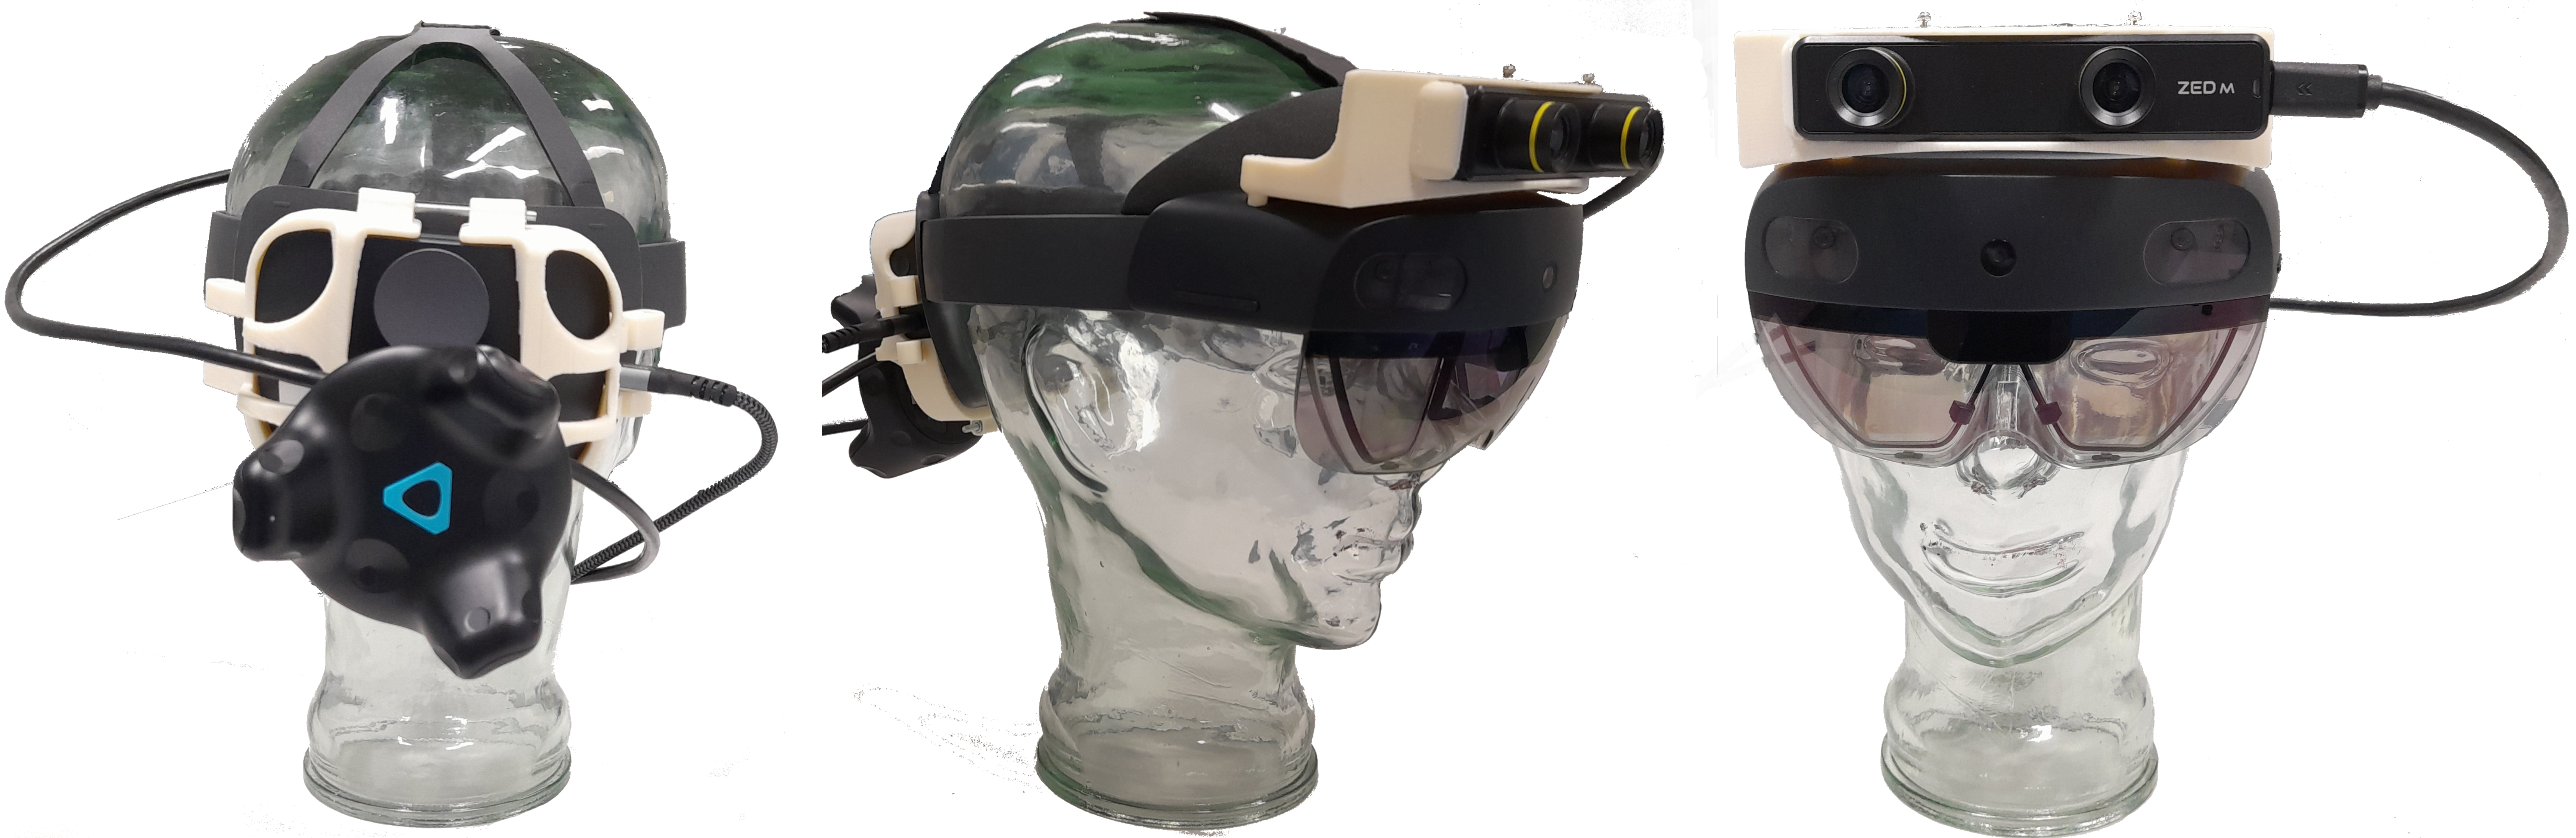
\includegraphics[width=0.9\columnwidth]{Chapter3/Images/HeadsetWithSensors.png}
    \caption{A image of the hardware used for this study on a glass mannequin head from three different angles.}
    \label{fig:X-ray Headset}
\end{figure}

% why the HoloLens was chosen over the Magic Leap
The choice of off-the-shelf devices for this study meant that it was not possible to take full advantage of some possible depth cues, specifically accommodation and convergence, since very few of the available headsets provide adequate accommodation.
I did consider the Magic Leap~\footnote{\url{https://www.magicleap.com}} as an alternative because it utilizes two focal planes, which would allow for some use of the accommodation depth cue. 
However, the two focal planes would have greatly complicated the setup this system would have required.
While the two depth planes of the Magic Leap were potentially useful, this technology would have complicated the camera pass-through to the user's vision and reduced the available frame rate, potentially causing issues for the study~\cite{Wang2023}.

\subsubsection{Vive Controller Set Up}
% What is the issue with using gestures in this study? 
The HoloLens 2 has an intuitive interaction design but has limited accuracy, especially at a distance.
MRTK utilizes Interpolation to create a smoother sense of motion within AR, making objects feel like they are drifting through the air. 
This works well for placing items in an approximate location but does not allow the participant to make precise controls, which is challenging. 
Generally, when using HoloLens2 to do this, it is recommended that you use long-distance motions for precise controls, but you would rather grab objects and place them. 
This was not an option, as participants could not touch the physical objects. 
So, a new system was built to view the participants' interactions. 

Rather than use the MRTK controls for this study, a Vive controller was utilized that controlled a ray out of the end of the controller, allowing participants to interact with the inside of the cube.
Using controllers enabled a more precise and predictable interaction than the default controls from MRTK. 
% Explaining how the Vive controller works
A separate VR system would be used to track the position of the Vive puck and controller.
It would then correct this position and transform it to be relative to where the puck should be relative to the HoloLens2, and send it to the main system as the position and rotation of the main controller.
%This allowed participants to interact with the virtual objects via the Vive controller. 
The system would then portray a ray coming out of the end of this controller. 
To lower the sensitivity of the Vive sensors and the HoloLens2 connection, a one-euro filter~\cite{Casiez2012} was used to remove any noise caused by the Vive's hardware that may be transmitted to the HoloLens2. 

\subsubsection{3D printed mounts} \label{sec:X-rayAddionalSensors}
To attach the sensors to the HoloLens2, 3D-printed mounts were required to fit comfortably onto the HoloLens2 with minimal movement due to head motions. This allowed the system to know where the camera was for each frame and where the controllers were located. Compared to the headset. Allowing for the controllers to be tracked in relation to the \gls{hmd}.

\begin{figure}[bt]
    \centering
    \includegraphics[width=0.9\columnwidth]{Chapter3/Images/RapidPrototypeing.jpg}
    \caption{A image of the prototype models developed to prototype the final ZED MINI camera mount}
    \label{fig:RapidPrototypeingZedHeadMount}
\end{figure}

% Technical
The Zed mini was required to capture as much of the participants' view as possible to locate it as close as possible to the users' eyes.
This meant the zed camera needed to be placed on top of the front of the HoloLens2, where two slots allow for the small items to be mounted.
To make this work, a keyhole-fit mechanism was utilized to hold these items in the same place without any chance of movement.
This required precise knowledge of the physical parameters of the HoloLens2. 
To be able to detect both the holes of the headset to establish that rapid prototyping was enacted, the development of a series of 3D printed models is required to try to determine the parameters of the HoloLens2 headset, which can be seen in figure \autoref{fig:HoloLens2Dimentions}.
The final version of this mount can is available open source~\footnote{\url{https://www.thingiverse.com/thing:4561113}}\textsuperscript{,}\footnote{\url{https://github.com/tomishninja/HoloLens2-Sensor-Mount-Repository}}

\begin{figure}[tb]
    \centering
    \includegraphics[width=0.9\columnwidth]{Chapter3/Images/HoloLens2Dimentions.png}
    \caption{A diagram of the base dimensions for the HoloLens2 calculated utilizing 3D prototyping. The top of the HoloLens2 Mount can be seen shaded in yellow.}
    \label{fig:HoloLens2Dimentions}
\end{figure}

The 3D-printed back Vive puck mount sat on the back of the HoloLens2 in \autoref{fig:X-ray Headset} was used to keep the Vive Puck visible and in the same place relative to the user.
This model was made open source to allow others to utilize this system~\footnote{\url{https://www.thingiverse.com/thing:4657299}}.
This design was created using photogrammetry. This version did not require such a complex design, and it acquired as many points of reference as possible to ensure the design's accuracy. 
This design utilized a two-piece system that could pressure clamp the mount if necessary to allow for more flexibility.
The areas of the design this would work with where could be found with the screw that could connect to a Vive puck as well as the top and bottom.
%The final design was built to be extendable if required, with two hinges on either side to allow for support if needed, but was deemed unnecessary and was removed in favor of having less weight.

\subsubsection{Environment and Apparatus}  \label{sec:X-ray Implmention Task And Reference}

\begin{figure}[tbp]
    \centering
    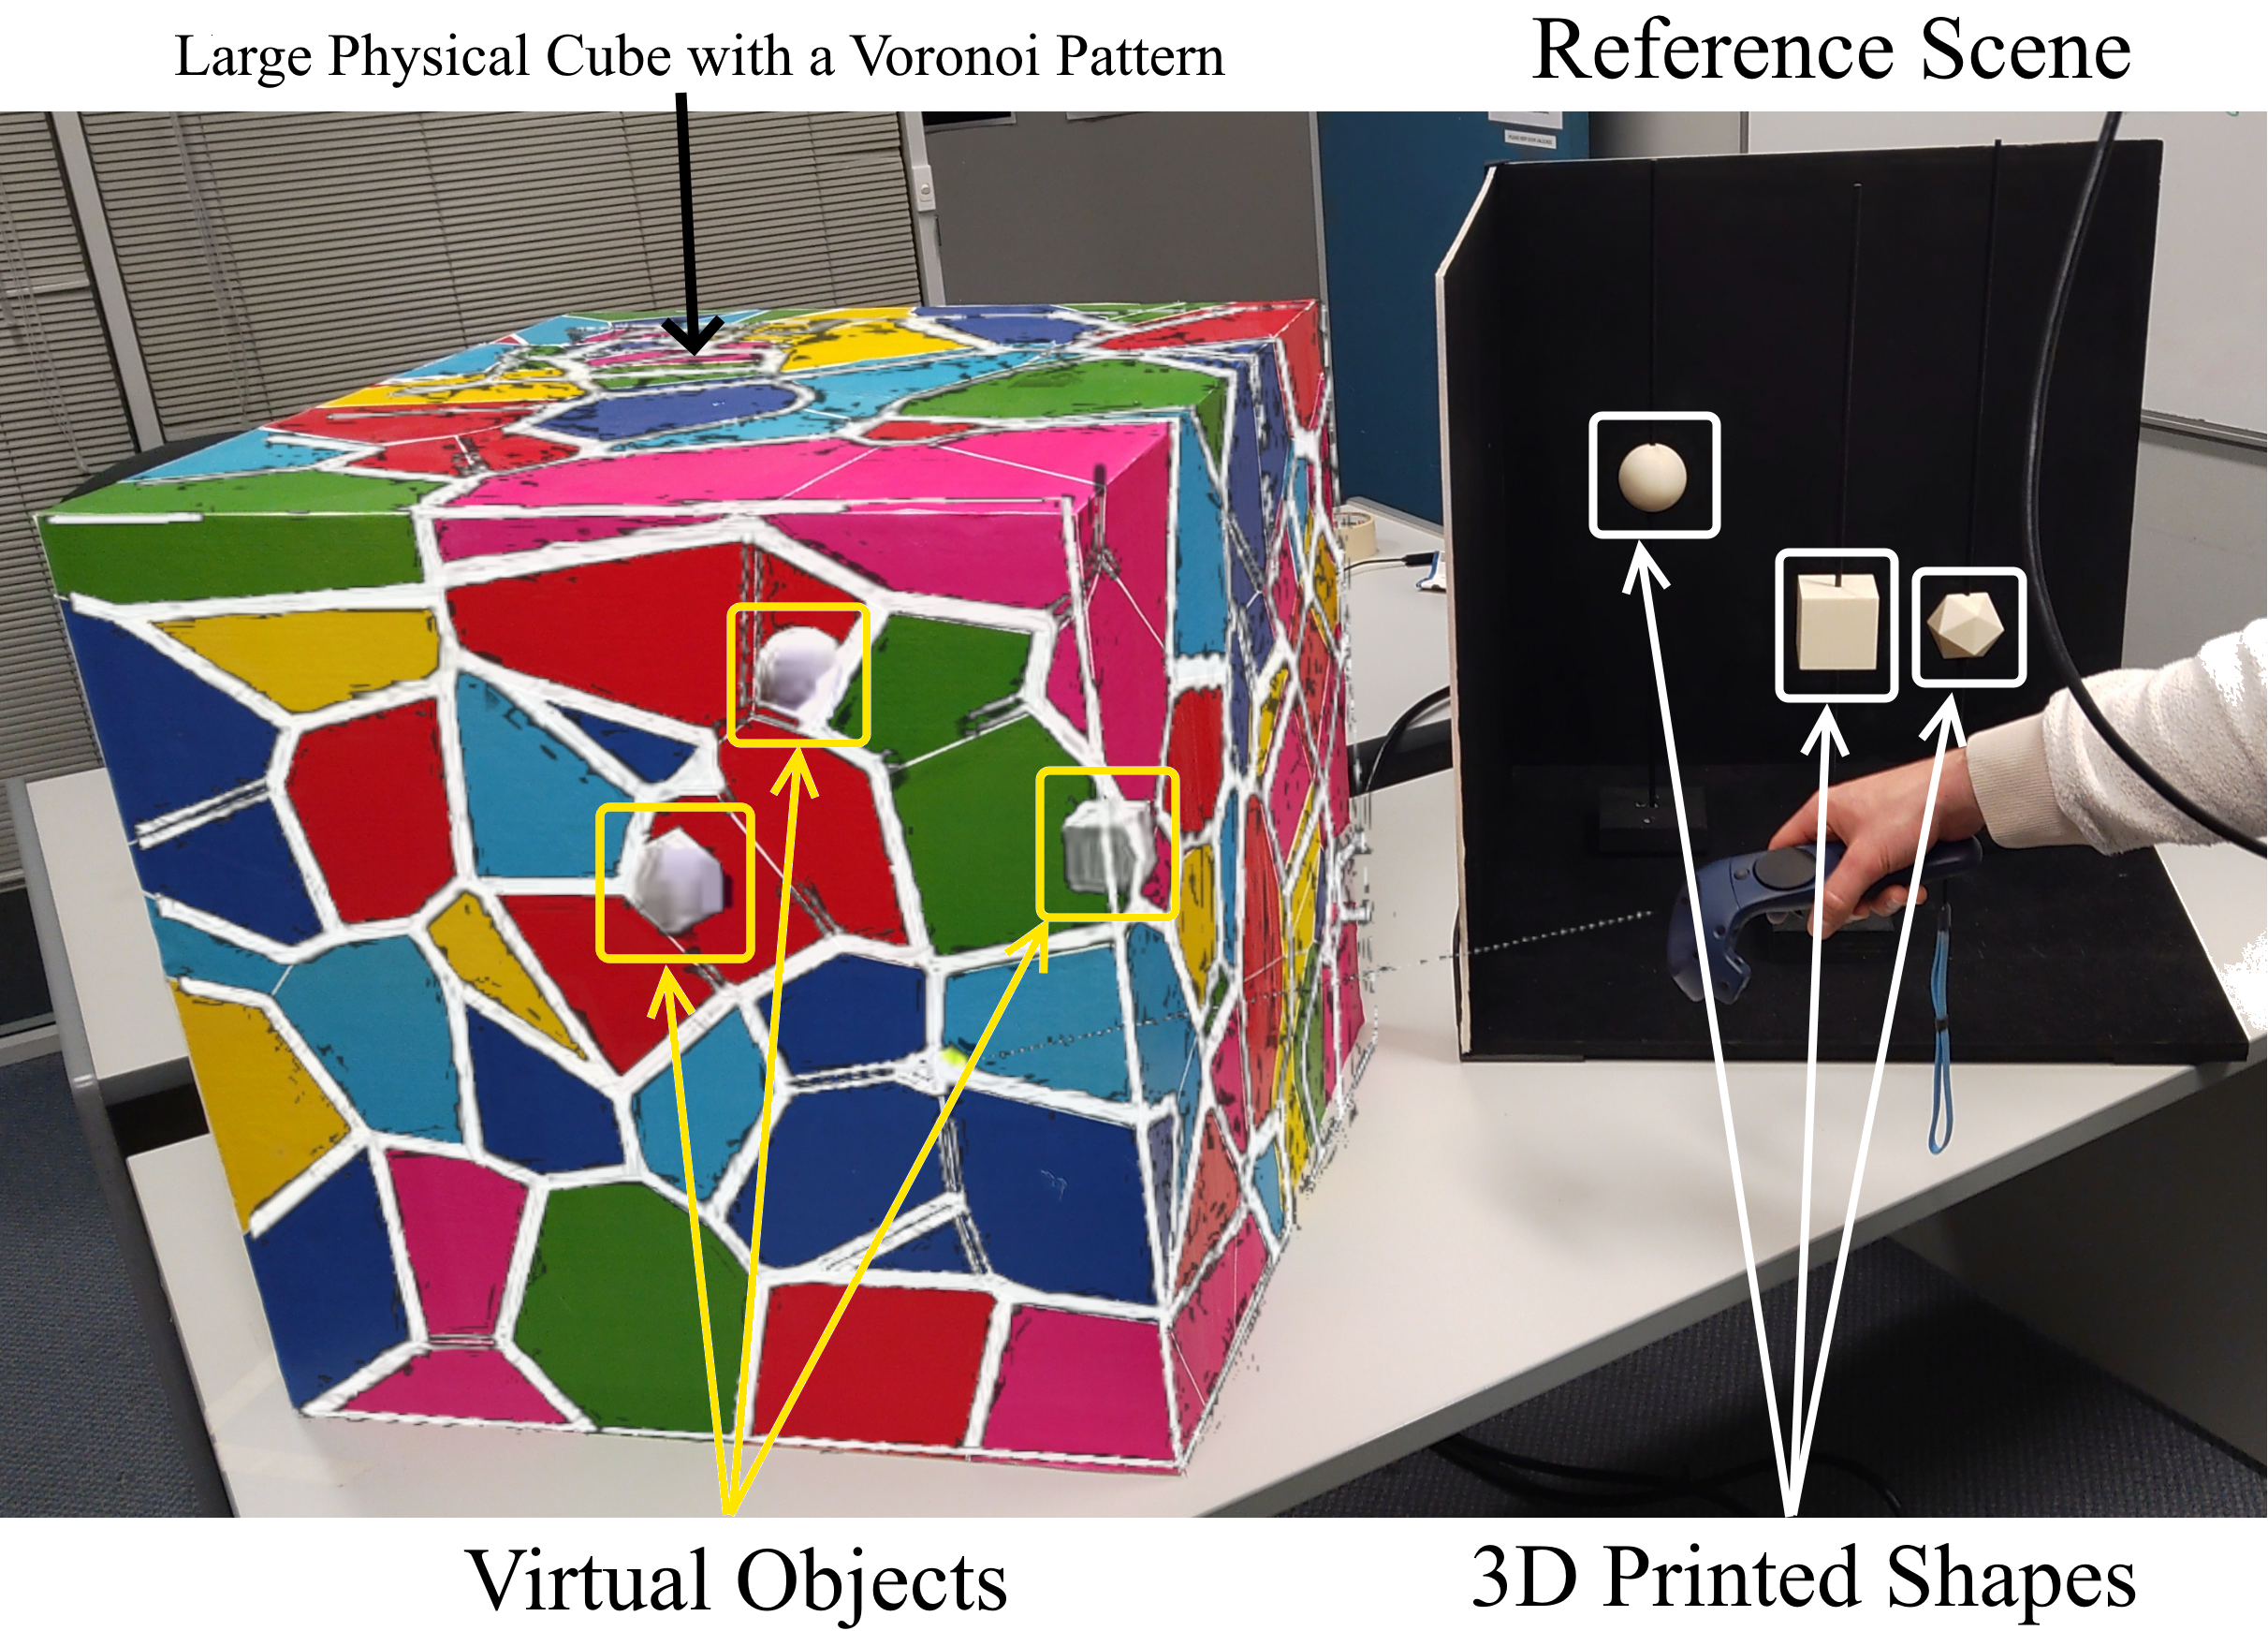
\includegraphics[width=0.9\columnwidth]{Chapter3/Images/UserStudyRunning (1).png}
    \caption[The study environment used for spatial estimation experiment.]{The study environment used for the spatial estimation experiment. Left is the large physical cube with a Voronoi pattern (for tracking) where \gls{X-ray Vision} techniques are performed. Right is a reference scene with movable 3D-printed objects that need replicating during the task.}
    \label{fig:Basic image of setup}
\end{figure}

% explaining the general physical environment
The physical study environment consisted of two cubes placed in an area where the participant could freely walk. The area where the participant could walk was constrained so that they were at most 1m from either of the physical scenes. The study area arrangement is depicted in \autoref{fig:Study One Set up}.

% a Deeper look into the cubes
The large Voronoi cube and reference scene, shown in \autoref{fig:Basic image of setup}, were very distinct in appearance, measuring 60cm along each axis.
The reference scene on the right-hand side of \autoref{fig:Basic image of setup} was the reference scene with a felt base. 
Smaller objects held up by stilts were placed in the cube that the participant would use as a reference.
The other large Voronoi cube was a brightly colored cube decorated in a Voronoi pattern designed to support \textit{Edge-Based} and \textit{Saliency} effects. 
This cube held the virtual objects displayed by the HoloLens2 that the user could interact with.

% Explain what these cubes did
The large physical cube with a Voronoi pattern was designed to be a 1:1 physical representation of the virtual world displayed in the brightly colored Voronoi cube. 
These cubes were designed to hold three geometric objects: a cube, a sphere, and an icosahedron.
The 3D-printed objects within the reference scene were ivory-colored to ensure that the shadows on the objects would be similar to the virtual ones displayed by the HoloLens2 and presented in the same orientation as the virtual objects. 
During the preliminary tests, no participant noted that the bright colors on the Voronoi cube were distracting.
Each stilt featured a square base measuring 100cm$^2$, which ensured that the center of each object was positioned at least 5cm away from any other object.
This enforced a minimum distance of 4 cm from any other object (except cube boundaries), ensuring that some spatial estimation was required to place the object.

% dimensions of the apparatuses
The geometric objects were identical in the physical reference scene and the virtual space. 
Each object had similar dimensions. 
The sphere (113.3cm$^3$) and the icosahedron (109.9cm$^3$) were made to be the largest size possible that would fit into the dimensions of the cube-shaped object (216cm$^3$).
The placement of each reference object was decided randomly along all axes while accounting for collisions and ensuring that each object was wholly within the cube.

\subsection{Study Variables} \label{sec:X-ray Design}
This section details the variables considered in this study. The independent variables are used to create each condition that will be tested throughout this study. The dependent variables will state the metrics that were required to track to answer the prior research questions. 

\subsubsection{Independent Variables} \label{sec:X-ray Design IV}
%This study utilized a 2 by 5 study design with both baselines (with no reference objects and no \gls{X-ray Visualization}. 

This study utilized a 2 by 5 design, with two separate baselines. 
The first baseline related to the presence of reference objects: participants either had no reference objects or two reference objects (a cube and a sphere) available in the scene (see \autoref{fig:Basic image of setup}). 
The second baseline related to visualization: participants either viewed the scene with one of four \gls{X-ray Visualization} techniques (\textit{Random Dot}, \textit{Tessellation}, \textit{Saliency}, \textit{Edge-Based}) or with no visualization at all (the baseline condition for this factor, \textit{None}).

Thus, the design contained two orthogonal baselines:
\begin{itemize}
    \item Reference baseline: no cube or sphere present.
    \item Visualization baseline: no \gls{X-ray Visualization} applied.
\end{itemize}

The conditions tested in this design are as follows:
\begin{itemize}
    \item (2) The presence of the reference objects: two reference objects (a cube and a sphere) and no reference objects (Shown in \autoref{fig:Basic image of setup}). 
    \item (5) X-ray visualization: \textit{Random Dot}, \textit{Tessellation}, \textit{Saliency}, \textit{Edge-Based} and \textit{None}. These were all previously mentioned and described in \autoref{sec:X-ray Vis}
\end{itemize}
\textbf{H.1} to \textbf{H.7} utilize both of these conditions, while \textbf{H.8} \& \textbf{H.9} only uses the \glspl{X-ray Visualization}.

\subsubsection{Dependent Variables}  \label{sec:X-ray Design DV}
The dependent variables state the different tracked measures utilized to confirm this research's hypotheses. 

\paragraph{Quantitative Variables}
\begin{itemize}
    \item \textbf{Accuracy}: Accuracy was measured as the distance between the center of the actual placement position and the center of the target position (\textbf{H.1}, \textbf{H.2}, \textbf{H.3} \& \textbf{H.4}).
    \item \textbf{Perspective Accuracy by axis}: Perspective accuracy was measured as the distance between the actual placement position (along the horizontal, vertical, and depth axes) and the target position from the participant's perspective at the time of placement (\textbf{H.2}, \textbf{H.3} \& \textbf{H.4}).
    \item \textbf{Time}: Overall time taken between the user starting the condition and the time the user chose to end the condition. The time the user spent holding the object for each condition was recorded (\textbf{H.5}). 
    \item \textbf{Distance Moved}: Throughout each task, data was gathered from the headset regarding the distance the headset was moved every frame. The total sum of this was used to determine how much various users felt the need to move around to get an understanding of various scenes (\textbf{H.6} \& \textbf{H.7}). 
    \item \textbf{Distance Icosahedron Was Moved}: For each task, users would be given as many opportunities to move the icosahedron as they felt necessary. Whenever the user moves the icosahedron, the distance it moves will be tracked similarly to its movement. Allowing for an assessment of the movement required to place the shape in every instance.
\end{itemize}

\paragraph{Subjective Variables}
\begin{itemize}
    \item \textbf{PAAS Questionnaire}: To gain an understanding of the possible cognitive loads undertaken via the various \gls{X-ray Visualization}s, the PAAS mental effort scale\cite{Paas1992} was utilized (\textbf{H.8}).
    \item \textbf{\gls{sus}}: A \gls{sus} questionnaire was utilized to determine how easy the various \gls{X-ray Visualization}s where to use (\textbf{H.8}).
    \item \textbf{Favorite \gls{X-ray Visualization}}: At the end of each study, users were asked to state what \gls{X-ray Visualization} was their favorite (\textbf{H.9}).
    \item \textbf{Comments and Feedback}: At the end of each study, users were asked to give feedback in the form of written text after completing the study  (\textbf{H.9}). 
\end{itemize}

\subsection{Task} \label{sec:X-ray User Study Procdedure}

\begin{figure}
    \centering
    \includegraphics[width=0.9\columnwidth]{Chapter3/Images/SkectchOfStudyAreaForStudy1.png}
    \caption[A top down view of the study setup for the spatial estimation experiment color coded in to the different areas of note]{A top down view of the study setup for the spatial estimation experiment color coded in to the different areas of note: a) Colourful Voronoi Cube; b) Black Inverse Reference  Cube; c) Area the participant could traverse; d) Examiner area; e) Main Processing Server; f) Projector setup; g) Vive sensors}
    \label{fig:Study One Set up}
\end{figure}

% Explaining the Vive setup
Participants were asked to perform a demographics survey at the start of each session. Then, they were asked to wear a HoloLens2 with an HTC Vive puck and a Zed mini mounted on it and given an HTC Vive controller for hand interactions with the study.
Allowing a pointer to come out of the controller to interact with the box's interior.
Participants were given a tutorial on how to use the controller for the task. 
This explanation included:
\begin{itemize}
    \itemsep-0.15em 
    \item When the pointer interacts with the icosahedron, it changes its color and surrounds the object with a transparent bubble.
    \item Using the touchpad on the controller, the ray cast could be grown (up to 1 meter in length) and shrunk as necessary. %, allowing the participants to interact within the box from any angle. 
    \item Participants could start and end each iteration by pressing the menu button on the Vive controller.
\end{itemize}

% Explaining the task the user had to do
Participants were instructed to place the virtual icosahedron in the same position in the Voronoi cube as the physical icosahedron was positioned in the physical reference scene. 
The other reference objects and their physical counterparts in the inverse cube were also pointed out to them. 
In each iteration of the study, one of four different \glspl{X-ray Visualization} or no visualization would be randomly chosen and shown on the outside of the cube. 
The initial position of the virtual icosahedron was at 5cm along all axes measured from the bottom front corner of the target Voronoi cube. 
If virtual reference objects were present for the iteration, they would be located at the correct relative position indicated by their physical counterparts.
All positions of the geometrical objects were generated before the study using a pseudo-random selection. 

A randomized order of conditions was used instead of a Latin balanced square. This choice was made to maintain flexibility in participant scheduling and accommodate uncertainty in recruitment numbers. Balanced Latin squares require fixed multiples of participants to achieve complete counterbalancing, which can become problematic when participant availability is unpredictable or when demographic representation is uneven. Randomization ensured that order effects were distributed across the sample while allowing the study to adapt to potential imbalances in participant demographics caused by pandemic-related constraints.

A \gls{sar} calibration guidance tool was used to position the physical objects in 3D space by the examiner within the reference scene~\cite{Bimber2004}.
The desired height position of each object was indicated using a wireframe representation of these models to ensure that they were in the correct position and facing the correct way.

% what the users were expected to do each time
During each task, the participants could freely move around the area shown in \autoref{fig:Study One Set up} but were not allowed to step outside the area.
Participants could reposition the icosahedron as often and as far as they wanted and had no time limit to complete the task.
This was aimed to reduce any pressure on the participants to complete the task quickly and allow them to focus on accuracy while also allowing them to move around the cube as much as they felt necessary focusing on how well they could perform the task with no restrictions, creating a more realistic experience.

% participant rigor
Participants were given three practice iterations of each task before data collection began.
Participants were given instructions and guidance during these practice iterations. 
Following the practice iterations, participants were presented with 10 iterations for each \gls{X-ray Visualization} effect. 
This would then be split into two randomly interleaved groups: one with two reference objects and one without any reference objects.
%Five of these would include two extra reference objects, and five would only include the icosahedron but no reference objects presented. 
After completing the ten iterations, the participant answered a visualization technique questionnaire, including a System Usability Survey~\cite{Brooke1996SUSA}, the PAAS subjective rating scale~\cite{Paas1992}, and several other custom questions. 
This procedure was repeated randomly for each \gls{X-ray Visualization} and the baseline condition.
In total, each participant spent an average of approximately 96 minutes ($\pm 61.52$) doing in this study, with the fastest participant spending about 31 minutes in the study and the slowest taking almost 4 hours and 21 minutes to complete this task. 

\section{Results}  \label{sec:X-ray Results}

\begin{figure*}[bt]
    \centering
    %\includesvg[width=\textwidth]{Chapter3/Images/DistanceToGoalGraphEffectOnlyVersion.svg
    %\includegraphics[width=\textwidth]{Chapter3/Images/AccuracyPlotOverallX-rayVision.pdf}
    \includegraphics[width=\textwidth]{Chapter3/Images/Impact of X-ray Visualization on Placement Accuracy.pdf}
    \caption[A graph representing the accuracy of participants' placement based on the distance the object was placed from the goal position within the large physical cube with a Voronoi pattern using the \glspl{X-ray Visualization}.]{
    A graph representing the accuracy of participants' placement based on the distance the object was placed from the goal position within the large physical cube with a Voronoi pattern using the \glspl{X-ray Visualization}. 
    The error bars indicate each condition's confidence levels (CL = 95\%).
    Significance differences are displayed as the lines on the top of the graph stars indicate significance (* = p $<$ 0.05; ** = p $<$ 0.01; *** = p $<$ 0.001).
    }
    \label{fig:X-ray Distance To Goal X-ray vision effect plot}
\end{figure*}


The analyses followed a within-group design, with a single group of participants completing all conditions (presence of reference objects and \glspl{X-ray Visualization}) to answer hypotheses \textbf{H.1} to \textbf{H.7}. 
\gls{lmm} was used to analyze the data, with participants as a random effect and the presence of reference objects and \glspl{X-ray Visualization} as fixed effects while allowing for repeated measures.
This allowed for the differences between each participant to be accounted for while still being able to analyze the effects of the independent variables


All results with a p-value $< 0.1$ are reported in this section. 
Any p-value $< 0.05$ is considered significant.
All results from the post hoc analysis in this section can be found in the appendix of this thesis. 

\subsection{Quantitative Results} \label{sec:X-ray Quantitative Results}
\begin{table*}[!b]
  \centering
  \scriptsize
  \addtolength{\tabcolsep}{-2.75pt}
  \caption[Table of \glspl{X-ray Visualization} used in this study. Showing the mean ($\mu$), standard deviation ($\sigma$), and the median (M) of the distance from the correct target position of all the \glspl{X-ray Visualization} from the user's sight.]{
  Table of \glspl{X-ray Visualization} used in this study. Showing the mean ($\mu$), standard deviation ($\sigma$), and the median (M) of the distance from the correct target position of all the \glspl{X-ray Visualization} from the user's sight (x, y, and z) and the distance to the goal (*). All measurements are in cm.
  %The top row of images shows the \glspl{X-ray Visualization} used in this study from the viewpoint of the HoloLens2's camera.
  The second column from the left indicates the presence of the reference objects (T indicates the presence of reference objects, while F indicates the absence of all reference objects in the scene).
  }


  \begin{tabular}{"c|c"c|c|c"c|c|c"c|c|c"c|c|c"c|c|c"}
    \cline{3-17}
    \multicolumn{2}{c"}{} & 
    \multicolumn{3}{c"}{Random Dot} & 
    \multicolumn{3}{c"}{Tessellation} &
    \multicolumn{3}{c"}{Edge-Based} & 
    \multicolumn{3}{c"}{Saliency} & 
    \multicolumn{3}{c"}{None} \\ 
    \cline{3-17}
    \multicolumn{2}{c"}{} & 
    $\mu$ & $\sigma$ & M & 
    $\mu$ & $\sigma$ & M & 
    $\mu$ & $\sigma$ & M & 
    $\mu$ & $\sigma$ & M & 
    $\mu$ & $\sigma$ & M \\ 
    \hline 
    \multirow{2}{*}{*)} & F 
    & 5.82 & 2.84 & 5.09
    & 5.47 & 2.38 & 5.25
    & 6.19 & 2.99 & 5.68 
    & 6.09 & 2.40 & 5.75 
    & 5.78 & 2.57 & 5.65  \\ 
    \cline{2-17} & T 
    & 4.24 & 1.97 & 4.09 
    & 4.58 & 2.18 & 4.30
    & 4.46 & 2.15 & 4.17 
    & 4.86 & 2.76 & 4.41 
    & 4.27 & 2.02 & 3.90  \\ 
    \hline 
    \multirow{2}{*}{x)} & F 
    & -0.69 & 3.19 & -0.88 
    & -0.08 & 3.34 & -0.24
    & -0.04 & 3.64 & 0.02 
    & -0.21 & 3.49 & -0.68 
    & -0.26 & 3.40 & -0.37  \\ 
    \cline{2-17} & T 
    & -0.19 & 2.86 & -0.16 
    & 0.07 & 3.35 & -0.31
    & 0.00 & 2.85 & -0.15 
    & 0.05 & 3.22 & -0.04 
    & 0.39 & 2.54 & 0.36  \\ 
    \hline 
    \multirow{2}{*}{y)} & F 
    & -0.98 & 2.90 & -0.98 
    & 0.03 & 3.05 & 0.09
    & -0.93 & 2.66 & -1.13 
    & -0.89 & 3.01 & -0.83 
    & -0.34 & 2.56 & -0.55  \\ 
    \cline{2-17} & T 
    & -0.46 & 2.22 & -0.21
    & -0.49 & 2.25 & -0.14
    & -0.26 & 2.36 & -0.03 
    & -0.79 & 2.36 & -0.56 
    & -0.07 & 2.56 & -0.12  \\ 
    \hline 
    \multirow{2}{*}{z)} & F 
    & 0.15 & 2.55 & 0.25 
    & -0.33 & 2.84 & -0.65
    & -0.76 & 3.21 & -0.84 
    & 0.00 & 3.18 & 0.24 
    & -0.48 & 2.84 & -0.89  \\ 
    \cline{2-17}  & T 
    & 0.02 & 2.32 & 0.27 
    & 0.17 & 2.13 & 0.15 
    & -0.59 & 2.35 & -1.15 
    & -0.08 & 2.96 & -0.61 
    & -0.00 & 2.37 & -0.04  \\ 
    \hline 
  \end{tabular}
  \label{tab:MeanAndMedianAccuracyValues}
\end{table*}

% \begin{figure}[tb]
%     \centering
%     %\includesvg[width=\textwidth]{Chapter3/Images/DistanceToGoalBasedOnUsersPerspectiveAndAxis.svg}
%     %\includegraphics[width=\textwidth]{Chapter3/Images/AccuracyPlotXAxisRefrenceObjects.pdf}
%     \includegraphics[width=\textwidth]{Chapter3/Images/Impact of Reference Objects on Placement Accuracy On X-axis.pdf}
%     \caption{
%         A graph representing the accuracy of participants' placement based on the distance the object was placed from the goal position on the X-axis within the large physical cube with a Voronoi pattern using the \glspl{X-ray Visualization}.
%         Positions were obtained from the final placement of the object.
%         The error bars indicate each X-ray visualization's confidence levels (CL = 95\%).
%     }
%     \label{fig:X-ray AccuracyPlotXAxis plot}
% \end{figure}

\begin{figure}[bt]
    \centering
    \includegraphics[width=\textwidth]{Chapter3/Images/Impact of X-ray Visualization on Placement Accuracy on the X axis.pdf}
    \caption[A Graphs representing the accuracy of participants' placement based on the distance they are from the goal position on the X-axis within the large, physical cube with a Voronoi pattern]{
    A Graphs representing the accuracy of participants' placement based on the distance they are from the goal position on the X-axis within the large, physical cube with a Voronoi pattern using the presence of the reference objects.
    Positions were obtained from the final placement of the object.
    The error bars indicate each condition's confidence levels (CL = 95\%).
    }
    \label{fig:X-ray AccuracyPlotXAxis plot}
\end{figure}

A \gls{lmm} was used to examine the differences across all variables measured within this section. 
\glspl{lmm} are now standard for analyzing repeated‐measures data in behavioral and cognitive experiments, because they allow for both fixed effects of experimental manipulations and random effects (e.g. subject‐level variability). 
This approach has several advantages over traditional methods such as ANOVA, including the ability to handle unbalanced data, account for individual differences, and model complex hierarchical structures~\cite{Meteyard2020, Bell2019, Singmann2019}.
Unlike traditional repeated-measures ANOVA, \glspl{lmm} are flexible to unbalanced data and missing observations, which was advantageous in this study context~\cite{Li2012a}.

\glspl{lmm} uses a similar method to linear regression ($y = X\beta + \varepsilon$) that is given fixed and random effects. Fixed Effects may not vary per condition; and random effects are estimated using $\beta \sim \mathcal{N} (\mu, \sigma^2)$, allowing the system to account for different variances between results of the random effect (mixed effects)~\cite{Models2006, Singmann2019}.
Overall, the model predicts the outcome variable (y) using a matrix of predictor variables (X) against a single column of fixed effects regression coefficients ($\beta$); The effect from the random effects (Z) is then multiplied to the random effect of a given fixed effect ($\gamma$), this value is then added against a vector column of the residuals values ($\varepsilon$) for each fixed effect. 
\[y = X\beta + Z\gamma + \varepsilon\]
This approach accounts for individual differences between participants in repeated measures on both normally distributed and non-normally distributed data and enables the examination of the effect of the number of objects~\cite{Kaptein2016, Adams2022, Cameron2005}.
The model was specified with the factors of the presence of virtual reference objects and \gls{X-ray Visualization} effect techniques, the dependent variable of the accuracy, viewpoint accuracy, distance moved, distance away, or time. 
The model was specified with fixed effects of x-ray visualization, the presence of reference objects, and an interaction effect between them, with a random effect of participants on the intercept. 
Significance values were extracted using Type II Wald chi-square tests using the following algorithm: 
\[ W = g(\hat{\theta})^{ \intercal } \left[ G V(\hat{\theta}) G^{\intercal} \right]^{-1} g(\hat{\theta})
\]
%Where G is the Jacobian matrix of $g(\theta)$ with respect to $\theta$, it's a matrix of partial derivatives of $g(\theta)$ the elements of each parameter.
Here, \( G \) denotes the Jacobian matrix of \( g(\theta) \) with respect to \( \theta \).
Each element of \( G \) represents the partial derivative of one component of \( g(\theta) \)
with respect to a corresponding parameter in \( \theta \), that is,
\[
G_{ij} = \frac{\partial g_i(\theta)}{\partial \theta_j}.
\]

pairwise post-hoc comparisons were conducted using Tukey’s \gls{hsd} for multiple comparisons to further validate p-values which is shown below:
\[ q = \frac{\bar{X}_i - \bar{X}_j}{\sqrt{\frac{MS_{\text{e}}}{n_{\text{t}}}}} \]
$q$ is the test statistic,
$\bar{X}_i - \bar{X}_j$ are the two groups being compared,
$MS_{\text{e}}$ is the mean square error from the groups calculated from the \gls{lmm},
$n_{\text{t}}$ is the total number of observations.

% \begin{figure}[tb]
%     \centering
%     %\includesvg[width=\textwidth]{Chapter3/Images/DistanceToGoalBasedOnUsersPerspectiveAndAxis.svg}
%     %\includegraphics[width=\textwidth]{Chapter3/Images/AccuracyPlotYAxisXRayVisionEffects.pdf}
%     \includegraphics[width=\textwidth]{Chapter3/Images/Impact of \gls{X-ray Visualization} on Placement Accuracy On Y-axis.pdf}
%     \caption{
%         A graph representing the accuracy of participants' placement based on the distance the object was placed from the goal position on the X-axis within the large cube with a Voronoi pattern using the \gls{X-ray Vision} visualizations.
%         Positions were obtained from the final placement of the object.
%         The error bars indicate each X-ray visualization's confidence levels (CL = 95\%).
%         %Significance differences are displayed as the lines on the right side of the graph stars indicate significance (* = p $<$ 0.05; ** = p $<$ 0.01; *** = p $<$ 0.001).
%     }
%     \label{fig:X-ray AccuracyPlotYAxis plot}
% \end{figure}

\begin{figure}[bt]
    \centering
    \includegraphics[width=\textwidth]{Chapter3/Images/Impact of X-ray Visualization on Placement Accuracy on the Y axis.pdf}
    \caption[Graphs representing the accuracy of participants' placement based on the distance they are from the goal position on the Y-axis within the large physical cube with a Voronoi pattern.]{
        Graphs representing the accuracy of participants' placement based on the distance they are from the goal position on the Y-axis within the large physical cube with a Voronoi pattern using either different (Right) \glspl{X-ray Visualization} or (Left) the presence of the reference objects.
        Positions were obtained from the final placement of the object.
        The error bars indicate each condition's confidence levels (CL = 95\%).}
    \label{fig:X-ray Reference Objects AccuracyPlotYAxis plot}
\end{figure}

\begin{figure*}[tb]
    \centering
    %\includesvg[width=\textwidth]{Chapter3/Images/DistanceToGoalBasedOnUsersPerspectiveAndAxis.svg}
    %\includegraphics[width=\textwidth]{Chapter3/Images/AccuracyPlotZAxisXRayVisionEffects.pdf}
    \includegraphics[width=\textwidth]{Chapter3/Images/Impact of X-ray Visualization on Placement Accuracy on the Z axis.pdf}
    \caption[Graphs representing the accuracy of participants' placement based on the distance the object was placed from the goal position on the Z-axis within the large physical cube with a Voronoi pattern]{
        Graphs representing the accuracy of participants' placement based on the distance the object was placed from the goal position on the Z-axis within the large physical cube with a Voronoi pattern using either different (Right) \glspl{X-ray Visualization} or (Left) the presence of the reference objects.
        The error bars indicate each X-ray visualization's confidence levels (CL = 95\%).
        Significance differences are displayed as the lines on the right side of the graph stars indicate significance (* = p $<$ 0.05; ** = p $<$ 0.01; *** = p $<$ 0.001).
    }
    \label{fig:X-ray AccuracyPlotZAxis plot}
\end{figure*}

% \begin{figure*}[bt]
%     \centering
%     %\includesvg[width=\textwidth]{Chapter3/Images/DistanceToGoalBasedOnUsersPerspectiveAndAxis.svg}
%     %\includegraphics[width=\textwidth]{Chapter3/Images/AccuracyPlotZAxisXRayVisionEffects.pdf}
%     \includegraphics[width=\textwidth]{Chapter3/Images/Impact of Reference Objects on Placement Accuracy On Z-axis.pdf}
%     \caption{
%         A Graph representing the accuracy of participants' placement based on the distance they are from the goal position on the Z-axis within the large physical cube with a Voronoi pattern using the presence of the reference objects.
%         The error bars indicate each condition's confidence levels (CL = 95\%).
%         Significance differences are displayed as the lines on the right side of the graph stars indicate significance (* = p $<$ 0.05; ** = p $<$ 0.01; *** = p $<$ 0.001).
%     }
%     \label{fig:X-ray AccuracyPlotZAxis plot}
% \end{figure*}

\subsubsection{Accuracy of Placement (H.1)} \label{sec:X-ray Quantitative Results Placement Accuracy}
%\paragraph{Distance To the Goal: }

Analysis of the accuracy of the user's placement of the virtual icosahedron object as compared to the target shape's position
% The model for the generic distance between the user's point of placement and the correct target position 
showed a significant fixed effect of the \gls{X-ray Visualization} effects ($\chi$2(4, N= 20) = 13.897, p  = 0.007) and the presence of the additional reference objects ($\chi$2(1, N= 20) = 77.641, p $<$ 0.0001), with no significant interaction effect. 

Post-hoc pairwise comparisons showed significantly improved accuracy when additional reference objects were present (p $<$ 0.0001, df = 989, t = 8.771), which can be seen on the right side of \autoref{fig:X-ray Distance To Goal X-ray vision effect plot}.
\textit{Saliency} showed significantly lower accuracy than \textit{None} (p = 0.0358, df = 989, t = -2.853), and \textit{Saliency} was also significantly less accurate than \textit{Tessellation} (p = 0.0414, df = 989, t = 2.8). 
The differences in placement accuracy using of different \gls{X-ray Vision} effects can be viewed in the left side of \autoref{fig:X-ray Distance To Goal X-ray vision effect plot}

\paragraph{Placement Accuracy from User Viewpoint by Axis (H.2 \& H.3):}
The placement accuracy of the virtual icosahedron object was also analyzed in relation to the participant's viewpoint at the time of placement.
The initial placement provides insight into how accurately an object can be positioned within a given space, allowing for measuring distance along each axis. This enables the determination of how precisely actions were perceived at the final moments of placement and helps isolate the areas most affected by different visualizations.

Positions were transformed into the relative space of the headset using its position and orientation matrix just after the user placed the object to compute the actual and correct final placement. The distance was then calculated along the three axes of the user's headset: the x-axis (horizontal) and y-axis (vertical) are the horizontal and vertical axis of the participant's view, respectively, and the z-axis was the direction the participant was looking.

The viewpoint accuracy on the x-axis, the \gls{lmm} showed users were significantly more accurate when the reference objects were present ($\chi$2(1, N= 20) = 5.6295, p  = 0.0184), while the \gls{X-ray Vision} effect ($\chi$2(4, N= 20) = 5.8363, p  = 0.2117) and the interaction effect ($\chi$2(4, N= 20) = 0.4646, p  = 0.9768) was not found to be significant.
The post-hoc comparison for the presence of reference objects showed a significant improvement in accuracy with reference objects present (p $=$ 0.0184, df = 989, t = -2.362). All these results can be seen in \autoref{fig:X-ray AccuracyPlotXAxis plot}. 

Regarding the viewpoint accuracy on the y-axis, the \gls{lmm} showed a significant difference between different \gls{X-ray Vision} effects ($\chi$2(4, N= 20) = 13.8972, p  = 0.0076) and no significance for the presence of reference objects($\chi$2(1, N= 20) = 77.6411, p  < 0.0001) and the interaction effect ($\chi$2(1, N= 20) = 5.1383, p  = 0.27340). 
The post-hoc comparisons between all of the \gls{X-ray Vision} effects showed no significant values.
There was some variability between \textit{None} and \textit{Saliency} (p = 0.0551, df = 989, t = 2.697) and \textit{Saliency} and \textit{Tessellation} (p = 0.0985, df = 989, t = -2.469). 
The left-hand side of \autoref{fig:X-ray Reference Objects AccuracyPlotYAxis plot} shows that where Saliency was slightly less accurate, but it was not significantly different.
Whereas, the right side of \autoref{fig:X-ray Reference Objects AccuracyPlotYAxis plot} does present some benefits to having reference objects in a scene. 

The viewpoint accuracy on the z-axis model showed a significant fixed effect of the \gls{X-ray Visualization} effects ($\chi$2(4, N= 20) = 11.9119, p $=$ 0.0066). The presence of the reference objects showed no significant effect ($\chi$2(1, N= 20) = 0.0002, p = 0.9878).
The interaction effect ($\chi$2(4, N= 20) = 2.5402, p = 0.6374) showed not significantly different.
The post-hoc effect showed that the \textit{Edge-Based} visualization was significantly less accurate at presenting depth than \textit{None} (p = 0.0499, df = 989, t = -2.734) and \textit{Saliency}(p = 0.0048, df = 989, t = -3.476).
Some variation could also be found when comparing \textit{Edge-Based} to \textit{Random Dot} (p = 0.0661, df = 989, t = -2.628) and \textit{Tessellation} (p = 0.0782, df = 989, t = -2.563). All these effects can be seen in \autoref{fig:X-ray AccuracyPlotZAxis plot}.

\begin{figure}[bt]
    \centering
    %\includesvg[width=\columnwidth]{Chapter3/Images/TimeRequiredToCompleteGraphChangedColor.svg}
    %\includegraphics[width=\columnwidth]{Chapter3/Images/TimeRequiredToCompleteReferenceObjects.pdf}
    %Impact of X-ray Visualization on the Time Required to Complete the Task.pdf
    \includegraphics[width=\columnwidth]{Chapter3/Images/Effect of the Time Required for Participants to Move the Icosahedron.pdf}
    \caption[Two box plots analyzing the time it took to complete the task compared between different (Right) \glspl{X-ray Visualization} and (Left) with and without the reference objects.]{
    Two box plots analyzing the time it took to complete the task compared between different (Right) \glspl{X-ray Visualization} and (Left) with and without the reference objects.
    The error bars indicate each condition's confidence levels (CL = 95\%).
    Significance differences are displayed as the lines on the right side of the graph stars indicate significance (* = p $<$ 0.05; ** = p $<$ 0.01; *** = p $<$ 0.001).
    }
    \label{fig:TimeRequiredToCompleteReferenceObjects}
\end{figure}

\subsection {Time Required (H.5)}
This section focuses on answering \textbf{H.5} in detail by looking at how long this task took between the different conditions and if this changed the quantity of time they spent moving the icosahedron around. 

\paragraph{Time Required for task completion (H.5): } \label{sec:X-ray Quantitative Results Placement Time}

% \begin{figure*}[tbp]
%     \centering
%     %\includesvg[width=\columnwidth]{Chapter3/Images/TimeRequiredToCompleteGraphChangedColor.svg}
%     %\includegraphics[width=\columnwidth]{Chapter3/Images/TimeRequiredToCompleteGraphXRayEffects.pdf}
%     \includegraphics[width=\columnwidth]{Chapter3/Images/Impact of \glspl{X-ray Visualization} and the Time Required to Complete the Task.pdf}
%     \caption{
%     A box plot analyzing the time it took to complete the task compared between different \glspl{X-ray Visualization}.
%     The error bars indicate each X-ray visualization's confidence levels (CL = 95\%).
%     Significance differences are displayed as the lines on the right side of the graph stars indicate significance (* = p $<$ 0.05; ** = p $<$ 0.01; *** = p $<$ 0.001).
%     }
%     \label{fig:TimeRequiredToCompleteGraphXRayEffects}
% \end{figure*}

% The amount of time each iteration took
The completion time for each iteration was measured from the time the participant pressed the start button until the time they pressed the end button. The model of completion time showed significant fixed effects of both the \gls{X-ray Visualization} effects ($\chi$2(4, N= 20) = 24.441, p $<$ 0.0001) and the presence of the reference objects ($\chi$2(1, N= 20) = 14.2427, p = 0.0002).
No significant interaction effect between \gls{X-ray Visualization} and the presence of the reference objects was found ($\chi$2(4, N= 20) = 2.4244, p = 0.6582).

Post-hoc pairwise comparisons of the \glspl{X-ray Visualization} showed \textit{None} was significantly faster than Edge (p $<$ 0.0001, df = 983, t = -4.693), \textit{Saliency} (p = 0.0039 df = 983, t = -3.536) and \textit{Tessellation} (p = 0.0396 df = 983, t = -2.817). Comparisons of the presence of reference objects showed participants were significantly slower with reference objects present (p = 0.0002, df = 989, t = -3.757).
These results and \autoref{fig:TimeRequiredToCompleteReferenceObjects} indicate that these \glspl{X-ray Visualization} may slow down the user slightly to allow them to achieve a similar level of accuracy. 

\paragraph{Time Participants Spent Moving the Object (H.5)} 
\begin{figure}
    \centering
    \includegraphics[width=\linewidth]{Chapter3/Images/Effect of Reference Objects onthe Participant's Movements.pdf}
    \caption[Graphs representing the percentage of time participants spent moving the icosahedron for each task for each \gls{X-ray Vision} effect.]{Graphs representing the percentage of time participants spent moving the icosahedron for each task for each \gls{X-ray Vision} effect and (Right) the percentage of time required to move the icosahedron that participants moved the icosahedron using either different (Right) \glspl{X-ray Visualization} or (Left) the presence of the reference objects.
    The error bars indicate each X-ray visualization's confidence levels (CL = 95\%).
    Significance differences are displayed as the lines on the right side of the graph stars indicate significance (* = p $<$ 0.05; ** = p $<$ 0.01; *** = p $<$ 0.001).}
    \label{fig:SpeedUserMovedObject}
\end{figure}

% \begin{figure}[tb]
%     \centering
%     \includegraphics[width=\columnwidth]{Chapter3/Images/Impact of Reference Objects on the Percentage of Time Participants Moved the Icosahedron.pdf}
%     \caption{
%     A box plot showing the number of percentage of time participants spent moving the icosahedron for each task for each X-ray vision effect
%     The error bars indicate each X-ray visualization's confidence levels (CL = 95\%).
%     Significance differences are displayed as the lines on the right side of the graph stars indicate significance (* = p $<$ 0.05; ** = p $<$ 0.01; *** = p $<$ 0.001).}
%     \label{fig:SpeedUserMovedObjectXray}
% \end{figure}

All of the times when a user would press the button to pick up an object and put the same object down were recorded and summarised across each task to record the time spent on each task.
This was calculated as a percentage of the time the participants moved the icosahedron each time.
This enabled the identification of which aspects of the task posed greater challenges for participants: placing the icosahedron or viewing and confirming its correctness.
The \gls{lmm} showed a significant fixed effect on the \gls{X-ray Visualization} condition ($\chi$2(4, N= 20) = 36.4188, p $<$ 0.0001) and the presence of the reference objects ($\chi$2(1, N= 20) = 7.7862, p = 0.005). No significant interaction effect was found. ($\chi$2(4, N= 20) = 4.9161, p = 0.296).

% \begin{figure}[tp]
%     \centering
%     \includegraphics[width=\columnwidth]{Chapter3/Images/Impact of Reference Objects on the Percentage of Time Participants Moved the Icosahedron.pdf}
%     \caption{
%     A box plot of percentage of time required to move the icosahedron that participants moved the icosahedron based on the presence of reference objects
%     The error bars indicate each condition's confidence levels (CL = 95\%).
%     Significance differences are displayed as the lines on the right side of the graph stars indicate significance (* = p $<$ 0.05; ** = p $<$ 0.01; *** = p $<$ 0.001).
%     }
%     \label{fig:SpeedUserMovedObjectReferenceObjects}
% \end{figure}

Post-hoc pairwise comparison of the \glspl{X-ray Visualization} showed participants held the object for significantly less time for \textit{Random Dot} than \textit{Edge} (p $=$ 0.0130, df = 989, t = -3.183), \textit{Tessellation} (p = 0.0364, df = 989, t = 2.847), and \textit{Saliency} (p $< 0.0001$, df = 989, t = 5.475), \textit{Edge} than for \textit{Saliency} (p = 0.0012, df = 983, t = 3.847), and \textit{None} than for \textit{Saliency} (p = 0.0012, df = 983, t = 3.847).
\autoref{fig:SpeedUserMovedObject} shows that the more occlusion a 
visualization had caused, the longer the participants were holding the icosahedron. %the more occlusion a visualization had caused the participants to hold the icosahedron longer.
Post-hoc comparisons of the presence of reference objects showed participants were significantly slower without reference objects present (p = 0.0056, df = 989, t = 2.778).

% \paragraph{Time Participants Spent Moving the Object} \label{sec:TimeSpentMovingTheObject}

% All of the times between when a user would press the button to pick up an object and put the same object down were recorded and summarised across each task to record how much time in each task.
% the \gls{lmm} showed a significant fixed effect the \gls{X-ray Visualization} condition ($\chi$2(4, N= 20) = 33.0345, p $<$ 0.0001).
% No significant effect regarding the presence of the reference objects ($\chi$2(1, N= 20) = 1.8470, p = 0.1741), and no significant interaction effect was found. ($\chi$2(4, N= 20) = 3.6116, p = 0.4611).

% \begin{figure}[tb]
%     \centering
%     %\includesvg[width=\columnwidth]{Chapter3/Images/PlotofSpeedUsersMovedTheObjectShowingX-rayvisionEffect.svg}
%     %\includegraphics[width=\columnwidth]{Chapter3/Images/TimeRequiredToPlaceThe IcosahedronX-rayVisionEffects.pdf}
%     \includegraphics[width=\columnwidth]{Chapter3/Images/Impact of \glspl{X-ray Visualization} on the Time Spent Moving Icosahedron.pdf}
%     \caption{
%     A box plot showing the number of seconds participants spent moving the icosahedron for each task for each X-ray vision effect
%     The error bars indicate each X-ray visualization's confidence levels (CL = 95\%).
%     Significance differences are displayed as the lines on the right side of the graph stars indicate significance (* = p $<$ 0.05; ** = p $<$ 0.01; *** = p $<$ 0.001).}
%     \label{fig:SpeedUserMovedObjectXray}
% \end{figure}

% Post-hoc pairwise comparison of the \glspl{X-ray Visualization} showed participants held the object for significantly less time for \textit{None} than \textit{Edge-Based} (p $=$ 0.0130, df = 989, t = -3.183), \textit{Random Dot} (p = 0.0364, df = 989, t = 2.847), and \textit{Saliency} (p $< 0.0001$, df = 989, t = 5.475). Users also moved significantly faster using \textit{Tessellation} than for \textit{Saliency} (p = 0.0012, df = 983, t = 3.847).
% Some variation was also found between Random Dot and Saliency (p = 0.0661, df = 989, t = -2.628), but it was insignificant.
% These differences can be seen in \autoref{fig:SpeedUserMovedObjectXray}.
% Post-hoc comparisons of the presence of reference objects showed participants were significantly slower without reference objects present (p = 0.0118, df = 989, t = 2.524), which can be seen in \autoref{fig:SpeedUserMovedObjectReferenceObjects}.

% \begin{figure}[tp]
%     \centering
%     %\includesvg[width=\columnwidth]{Chapter3/Images/PlotofSpeedUsersMovedTheObjectShowingReferenceObject.svg}
%     %\includegraphics[width=\columnwidth]{Chapter3/Images/TimeRequiredToCompleteGraphReferenceObject.pdf}
%     \includegraphics[width=\columnwidth]{Chapter3/Images/Impact of Reference Objects on the Time Spent Moving Icosahedron.pdf}
%     \caption{
%     A box plot of Time required to move the icosahedron that participants moved the icosahedron based on the presence of reference objects
%     The error bars indicate each X-ray visualization's confidence levels (CL = 95\%).
%     Significance differences are displayed as the lines on the right side of the graph stars indicate significance (* = p $<$ 0.05; ** = p $<$ 0.01; *** = p $<$ 0.001).
%     }
%     \label{fig:SpeedUserMovedObjectReferenceObjects}
% \end{figure}

%
% % Removing this and instead looking at the speed the user could interact with this object.
% % but the comparison between the results is interesting
%
% \paragraph{Amount Icosahedron was Moved} \label{sec:X-ray Quantitative Results Time The Object was hold}

% \begin{figure}[tb]
%     \centering
%     %\includesvg[width=\columnwidth]{Chapter3/Images/TimeRequiredToPlaceIcosahedron.svg}
%     %\includegraphics[width=\columnwidth]{Chapter3/Images/AmountOfMovmentToPlaceIcosahedron.pdf}
%      \includegraphics[width=\columnwidth]{Chapter3/Images/Impacted}
%     \caption{The amount participants moved the Icsoahedron during each iteration}
%     \label{fig:SpeedUserMovedObjectXray}
% \end{figure}
% % The time users moved the held item
% In addition to completion time, the duration the user spent holding the object was also analyzed. The \gls{lmm} showed a significant fixed effect between the x-ray vision effects ($\chi$2(1, N= 20) = 25.3929, p $<$ 0.0001). No significant effect was shown regarding the reference objects or ($\chi$2(4, N= 20) = 0.0014, p = 0.9702),
% and no significant interaction effect was found. ($\chi$2(4, N= 20) = 4.7149, p = 0.3178). 

% Post-hoc pairwise comparison of the \glspl{X-ray Visualization} showed participants moved the icosahedron for significantly less time between \textit{Saliency}, and \textit{None} (p $<$ 0.0001, df = 989, t = 4.903) and \textit{Random Dot} (p = 0.0364, df = 989, t = 3.352), and \textit{Saliency} (p = 0.0074, df = 989, t = -5.475). Some variation was also noticed between for \textit{Tessellation} than for \textit{Saliency} (p = 0.0012, df = 989, t = -3.847), and \textit{Saliency} and \textit{Edge-Based} (p = 0.0721, df = 989, t = -2.595). These comparisons can be viewed in \autoref{fig:SpeedUserMovedObjectXray}.



% \begin{figure}[!bthp]
%     \centering
%     %\includesvg[width=\columnwidth]{Chapter3/Images/s.svg}
%     \includegraphics[width=\columnwidth]{Chapter3/Images/Impact of Reference Objects on the Participant's Movements.pdf}
%     \caption{
%         The distance participants walked for each iteration was based on the differences between each \gls{X-ray Visualization} they were experiancing.
%         The error bars indicate each X-ray visualization's confidence levels (CL = 95\%).
%         Significance differences are displayed as the lines on the right side of the graph stars indicate significance (* = p $<$ 0.05; ** = p $<$ 0.01; *** = p $<$ 0.001).
%     }
%     \label{fig:DistanceMoved}
% \end{figure}

\begin{figure}[!bt]
    \centering
    \includegraphics[width=\columnwidth]{Chapter3/Images/Effect of Reference Objects onthe Participant's Movements V1.pdf}
    \caption[The distance participants walked for each when (Left) different \glspl{X-ray Visualization} were displayed to them or (Right) the differences when reference objects were or were not available.]{
        The distance participants walked for each when (Left) different \glspl{X-ray Visualization} were displayed to them or (Right) the differences when reference objects were or were not available.
        The error bars indicate each X-ray visualization's confidence levels (CL = 95\%).
        Significance differences are displayed as the lines on the right side of the graph stars indicate significance (* = p $<$ 0.05; ** = p $<$ 0.01; *** = p $<$ 0.001).
    }
    \label{fig:DistanceMoved}
\end{figure}

\subsubsection{User Behaviour Results (H.6 \& H.7)} \label{sec:UserBehaviourResults}
This section is focused on how the different conditions affected the participant's ability to move around the environment and where they felt comfortable standing. 


\paragraph{Distance Moved (H.6):} \label{sec:X-ray Quantitative Results DistanceMoved}

The \gls{lmm} for the distance moved throughout each iteration by the participants showed a significant fixed effect between the \gls{X-ray Visualization} effects ($\chi$2(4, N= 20) = 52.8212, p $= 0.0043$) and a significant difference between the presence of the virtual reference objects ($\chi$2(1, N= 20) = 7.8110, p = 0.0052). Still, no significant interaction effect between the \gls{X-ray Visualization} effect and the presence of the reference objects was found $\chi$2(4, N= 20) = 0.4301, p = 0.9799.
Post-hoc pairwise comparisons found that users moved significantly more when the reference objects were present (p = 0.0055, df = 989, t = -2.782).
Comparisons of the combined \gls{X-ray Visualization} effects and the presence of the reference objects showed significance between the \textit{Edge-Based} and \textit{Saliency} Visualizations (p $=$ 0.003, df = 989, t $=$ 3.610) as well as some variance between \textit{Edge-Based} and \textit{Saliency} (p $<$ 0.0806, df = 989, t $=$ 2.550), and \textit{Random Dot} and \textit{Saliency} (p $<$ 0.0957, df = 989, t $<$ 2.481) but no significance.
Plots illustrating these effects can be seen in \autoref{fig:DistanceMoved}.

% \begin{figure}[!btp]
%     \centering
%     %\includesvg[width=\columnwidth]{Chapter3/Images/DistanceTraveledViolinPlot.svg}
%     %\includegraphics[width=\columnwidth]{Chapter3/Images/DistanceUsersMovedDuringTheTaskReference Objects.pdf}
%     \includegraphics[width=\columnwidth]{Chapter3/Images/Impact of Reference Objects on the Participant's Movements.pdf}
%     \caption{
%         The distance participants walked for each iteration was based on the differences when reference objects were or were not available.
%         The error bars indicate each condition's confidence levels (CL = 95\%).
%         Significance differences are displayed as the lines on the right side of the graph stars indicate significance (* = p $<$ 0.05; ** = p $<$ 0.01; *** = p $<$ 0.001).
%     }
%     \label{fig:DistanceUsersMovedDuringTheTaskReference}
% \end{figure}

\paragraph{Distance from Box (H.7)} \label{sec:X-ray Quantitative Results Distance Stood Away From the Box}
\begin{figure}[!btp]
    \centering
    %\includesvg[width=\columnwidth]{Chapter3/Images/DistanceTraveledViolinPlot.svg}
    %\includegraphics[width=\columnwidth]{Chapter3/Images/DistanceUsersMovedDuringTheTaskReference Objects.pdf}
    %\includegraphics[width=\columnwidth]{Chapter3/Images/Impact of Reference Objects on Participant Distance from Colorful Voronoi Box.pdf}
    \includegraphics[width=\columnwidth]{Chapter3/Images/Impact of Reference Objects on Participant Distance from Colorful Voronoi Box.pdf}
    \caption[Box plots represent the distance participants walked for each iteration.]{
        The distance participants walked for each iteration was based on the differences between (Right) each \gls{X-ray Visualization} they expressed or (Left) when reference objects were unavailable.
        The error bars indicate each condition's confidence levels (CL = 95\%).
        Significance differences are displayed as the lines on the right side of the graph stars indicate significance (* = p $<$ 0.05; ** = p $<$ 0.01; *** = p $<$ 0.001).
    }
    \label{fig:DistanceAwayFromBox}
\end{figure}

The \gls{lmm} of the distance the participants stood away from the large physical cube throughout the task on average showed a significant fixed effect of the \gls{X-ray Visualization} effects ($\chi$2(1, N= 20) = 14.1305, p $=$ 0.0067). Both the presence of reference objects ($\chi$2(4, N= 20) = 0.5301, p $=$ 0.4666) and the interaction effects these ($\chi$2(4, N= 20) = 0.5013, p $=$ 0.9733) showed no significance.
Post-hoc pairwise comparisons of the \gls{X-ray Visualization} effects showed a significant result between \textit{Random Dot} and \textit{saliency} (p $=$ 0.0217, df = 989, t $=$ 3.021). 
Some variation was found between \textit{Edge-Based} and \textit{Random Dot} (p $=$ 0.0875, df = 989, t $=$ -2.716) and \textit{None} and \textit{Saliency}  (p $=$ 0.0652, df = 989, t $=$ 2.633) but no significance. Comparisons between \gls{X-ray Vision} effects can be seen on the right side of \autoref{fig:DistanceAwayFromBox}.

% \begin{figure}[tb]
%     \centering
%     \includegraphics[width=\columnwidth]{Chapter3/Images/X-ray Visualization on Participant Distance from Colorful Voronoi Box.pdf}
%     \caption{
%         The distance average distance participants stood away from the large Voronoi box for each iteration was based on the differences between each \gls{X-ray Visualization} they were experiencing.
%         The error bars indicate each X-ray visualization's confidence levels (CL = 95\%).
%         Significance differences are displayed as the lines on the right side of the graph stars indicate significance (* = p $<$ 0.05; ** = p $<$ 0.01; *** = p $<$ 0.001).
%     }
%     \label{fig:DistanceAwayFromBox}
% \end{figure}

\paragraph{Speed Object Was Moved (H.6)}\label{Sec: speed user move the object}

% \begin{figure}[tb]
%     \centering
%     \includegraphics[width=\columnwidth]{Chapter3/Images/Impact of \glspl{X-ray Visualization} on the Velocity Participants Moved the Icosahedron.pdf}
%     \caption{
%         A box plot representing the speed/velocity in which the object was moved based on the icosahedron between each \gls{X-ray Visualization} they were experiencing.
%         The error bars indicate each X-ray visualization's confidence levels (CL = 95\%).
%         Significance differences are displayed as the lines on the right side of the graph stars indicate significance (* = p $<$ 0.05; ** = p $<$ 0.01; *** = p $<$ 0.001).
%     }
%     \label{fig:}
% \end{figure}

The speed at which the users moved the item was also measured by the sum of the times the user moved the object divided by the amount of distance the icosahedron would have been moved.
Understanding this provides insights into when participants felt confident in selecting a location for the icosahedron or whether the visualization enhanced their spatial awareness.
The \gls{lmm} showed a significant fixed effect between the \gls{X-ray Vision} effects ($\chi$2(1, N= 20) = 18.2724, p $=$ 0.0015) and a significant fixed effect was shown regarding the reference objects ($\chi$2(4, N= 20) = 8.9925, p = 0.0097). No significant interaction effect was found. ($\chi$2(4, N= 20) = 1.8465, p = 0.764). 

Post-hoc pairwise comparisons found users movement was both significantly different and faster when reference objects were present (p = 0.0102, df = 989, t = 2.574), which can be seen in \autoref{fig:WithReferenceObjects}.
The post-hoc comparisons for the \gls{X-ray Vision} effects show that \textit{Random Dot} was significantly faster both than \textit{Saliency} (p = 0.0017, df = 989, t = -3.754) and \textit{Tessellation} (p = 0.0088, df = 989, t = -3.303), which can be seen in \autoref{fig:WithReferenceObjects}.

\begin{figure}[bt]
    \centering
    \includegraphics[width=\columnwidth]{Chapter3/Images/Impact of Reference Objects on the Velocity Participants Moved the Icosahedron.pdf}
    \caption[Box plots representing the speed/velocity in which the object was moved based on the icosahedron.]{
        Box plots representing the speed/velocity in which the object was moved based on the icosahedron: (Left) between each \gls{X-ray Visualization} they were experiencing or (Right) whether reference objects were present.
        The error bars indicate each condition's confidence levels (CL = 95\%).
        Significance differences are displayed as the lines on the right side of the graph stars indicate significance (* = p $<$ 0.05; ** = p $<$ 0.01; *** = p $<$ 0.001).
    }
    \label{fig:WithReferenceObjects}
\end{figure}

\subsection{Subjective  Results (H.8 \& H.9)} \label{sec:X-ray Subjective Results}
% \begin{figure}[htp]
%     \centering
%     \includegraphics[width=\columnwidth]{Chapter3/Images/XrayPaasResults.pdf}
%     \caption{A bar plot showing PAAS cognitive load results acquired after each participant finished using an \gls{X-ray Visualization} in the study. Higher scores indicate a higher cognitive load required. Error bars indicate $\pm$ standard deviation.}
%     \label{fig:Study 1 PASS Reslts Plot}
% \end{figure}

This section focuses on answering \textbf{H.8} and \textbf{H.9} in detail by looking at the subjective data collected throughout the study.
All subjective data was found to be non-normally distributed using a Shapiro-Wilk test (p $<$ 0.05). 
Therefore, a non-parametric Friedman test was used to determine if there were any significant differences between the various conditions.
Mixed Effect Models were not used since the data was represents the participant's subjective opinion of each condition rather than a measurable quantity as such treatment of the participant as a random effect was not necessary.

The PAAS results (shown in the upper left plot of \autoref{fig:SubjectivePlots}) showed a significant difference between the \glspl{X-ray Visualization} using a Friedman rank sum test
($\chi$2(4, N= 20) = 41.185, p $<$ 0.0001).
Post-hoc analysis with pairwise Wilcoxon signed-rank tests was conducted with a Bonferroni correction applied. 
Comparisons showed significantly increased cognitive load between 
\textit{Saliency} and \textit{Edge-Based} (p = 0.0208),
\textit{Saliency} and \textit{None} (p $<$ 0.0001),
\textit{Saliency} and \textit{Random Dot} (p = 0.0003),
\textit{Saliency} and \textit{Tessellation} (p $<$ 0.0001).

\begin{figure}[htp]
    \centering
    \includegraphics[width=\linewidth]{Chapter3/Images/SubjectiveGraphs.pdf}
    \caption[Three plots displaying the subjective results collected throughout the course of this study.]{Three plots displaying the subjective results collected throughout the course of this study. 
    (Upper Left) PAAS cognitive load results were acquired after each participant finished using an \gls{X-ray Visualization} in the study. Higher scores indicate a higher cognitive load required.
    (Lower Left) The System Usability Scale (SUS) results were acquired after each participant finished using an \gls{X-ray Visualization} in the study. Higher scores indicate better usability.
    (Right) A tally of participants' favorite visualizations was totaled by having them choose their favorite ones. Error bars show standard error values.
    Error bars indicate $\pm$ standard deviation. Significance differences are displayed as the lines on the right side of the graph stars indicate significance (* = p $<$ 0.05; ** = p $<$ 0.01; *** = p $<$ 0.001).
    }
    \label{fig:SubjectivePlots}
\end{figure}

% A chi-square showed highly there was a significant relationship between different visualizations and the users confidence  $\chi$2(4, N= 20) = 61.495, p $<$ 0.00001,
% \textit{Saliency} was found to be much lower than the other other visualizations. 

%
%Kendalls's rank correlation was conducted to determine if the final Sus Scores.
%The SUS scores between \gls{X-ray Vision} effects and the final SUS scores showed no correlation.
The System Usability Scale results (shown in the lower left of \autoref{fig:SubjectivePlots}) showed a significant difference between the \glspl{X-ray Visualization} using a Friedman rank sum test
$\chi$2(4, N= 20) = 45.234, p $<$ 0.0001.
Post-hoc analysis with pairwise Wilcoxon signed-rank tests was conducted with a Bonferroni correction applied, resulting in a significantly lower usability score for \textit{Saliency} than \textit{Edge-Based} ($p = 0.0012$), \textit{None} ($p = 0.0002$), \textit{Random Dot} ($p = 0.0002$), and \textit{Tessellation} ($p = 0.0002$).

% \begin{figure}[btp]
%     \centering
%     \includegraphics[width=\columnwidth]{Chapter3/Images/XraySusResults.pdf}
%     \caption{A box plot showing the System Usability Scale (SUS) results acquired after each participant finished using an \gls{X-ray Visualization} in the study. higher scores indicate better usability. Error bars indicate $\pm$ standard deviation.}
%     \label{fig:SUS Reslts Plot}
% \end{figure}

At the end of each study, users were asked if they could state their favorite visualization and explain why. The results are tallied and displayed the results in the right-hand side plot in \autoref{fig:SubjectivePlots}. 
No significant difference was found between the \gls{X-ray Vision} effects when using a Chi-Square Test $\chi$2(4, N= 20) = 2.5, p $=$ 0.6446 when participants where asked why this visualization seems to have been their favorite. The results can be seen in \Cref{app:Chapter3Comments}. 

Participants would seem to have picked \textit{Tessellation} and \textit{None} more often as they were less occlusive and did not interfere with the task. \textit{Tessleation} seems to have provided users with enough visual cues to be able to navigate with it easily, making it the second most preferred method of visualizing the internal structures of an element. Users also reported liking \textit{Random Dot} since its design matched the shape of the box the most. User comments found in \Cref{app:Chapter3Comments} show that \textit{Saliency} was criticized for blocking out too much of the object underneath. At the same time, several participants liked how unobtrusive the edge-based visualization was, but some participants noticed a slight delay while using both it and \textit{Saliency}.


% \begin{figure}[btp]
%     \centering
%     \includegraphics[width=\columnwidth]{Chapter3/Images/FavoriteXrayVis.pdf}
%     \caption{
%         This bar chart shows a tally of participants' favorite visualizations, which was totaled by having them choose their favorite ones. Error bars show standard error values
%     }
%     \label{fig:plotsOfFavoritevisualizations}
% \end{figure}

\section {Discussion}  \label{sec:X-ray Discussion}
The findings from \autoref{sec:X-ray Results} present a broad spectrum of findings, which this section discusses in detail.
Notably, it was found that while \textit{Saliency} was beneficial for depth perception, it hindered the general placement of objects and was generally found to be the hardest to use when evaluating its usability and participants' cognitive loads.

%H.1 Participants will place the virtual icosahedron closer to the correct target position when they are using the Saliency visualization.
%H.2 Participants’ vertical and horizontal placement of the virtual icosahedron will be further from the correct target position when using the Saliency visualization.
%H.3 Participants’’ depth-based placement of the virtual icosahedron closer to the correct target position when they are using the Saliency visualization.
\subsection{Accuracy of Placement (H.1)}
The results shown in \autoref{sec:X-ray Quantitative Results Placement Accuracy} from this study did not support hypothesis one but partially supported hypothesis three. The right-hand side of \autoref{fig:X-ray AccuracyPlotZAxis plot} shows \textit{Saliency} positively affected depth perception compared to the edge-based visualization.
\autoref{tab:MeanAndMedianAccuracyValues} shows that while there seems to be a lot of difference between \textit{Saliency's} median and mean values being over 3 cm different, whereas other conditions throughout this study were relatively consistent.
This shows that users were very inconsistent with saliency, with their results sometimes being very accurate and sometimes being very inaccurate. 
This is likely because the occlusion created by the saliency covered larger areas of the visualization, showing that more occlusion can lead to better depth perception.

\subsection{Placement Accuracy from User Viewpoint by Axis (H.2 \& H.3)}
The right-hand side of \autoref{fig:X-ray AccuracyPlotXAxis plot} shows that \textit{Saliency} was the least accurate visualization on the horizontal axis. 
This can be explained better in-depth when looking at insignificant trends on the vertical axis (shown in \autoref{fig:X-ray Reference Objects AccuracyPlotYAxis plot}) and the values for x and y in \autoref{tab:MeanAndMedianAccuracyValues} where both random dot and saliency show a worse mean and standard deviation values.
This is likely due to the high occlusion in this X-ray visualization.
The effects that occluded the least gave the user a better understanding of space, where the shapes were inside the large physical cube with a Voronoi pattern. 
Still, the results from \autoref{fig:X-ray AccuracyPlotXAxis plot} and \autoref{fig:X-ray Reference Objects AccuracyPlotYAxis plot} lacked the significance to support hypothesis two. 

%The results in \autoref{sec:X-ray Quantitative Results Placement Accuracy} and \autoref{tab:MeanAndMedianAccuracyValues} seem to indicate that when using an OST AR device, the edge-based visualization provides the worst depth perception objects when it is not being used with the reference objects there are no reference objects to view. 
The results in \autoref{sec:X-ray Quantitative Results Placement Accuracy} and \autoref{tab:MeanAndMedianAccuracyValues} indicate that, on an \gls{ost} \gls{ar} device, the edge-based visualization produced the poorest depth perception, particularly when no reference objects were present.
This could be due to two reasons: as mentioned previously, prior work has shown that more occlusion allows for better depth perception~\cite{Otsuki2017}, provided the visualization does not occlude too much~\cite{Santos2016}; the other reason may be due to the edge-based visualization in this instance doesn’t represent the shape of the cube well due to the mosaic nature of the pattern~\cite{Avery2009}. 
For this research, a Voronoi effect was chosen to be used on the large physical cube, as I hypothesized to aid both the \textit{Saliency} and \textit{Edge-Based} \gls{X-ray Vision} effects by creating more areas for them to highlight; however, due to the non-uniform pattern on the box, the fact participants were looking down at it and within the box and rather all may show a weakness in this format when compared to a brick wall~\cite{Avery2009, Sandor2010}. 
Previous studies indicate \textit{Edge-Based} visualization can tell a user if an object is in front of or behind another object quite well~\cite{Kalkofen2007, Avery2009, Zollmann2014}. Still, the results from this study indicate the impact on depth perception can be slightly misleading. 
These findings may also be true for the \textit{Saliency} visualization; however, the improvement which can be seen in \autoref{fig:X-ray AccuracyPlotZAxis plot} and lowest mean accuracy showed in \autoref{tab:MeanAndMedianAccuracyValues} illustrates that the depth perception \textit{Saliency} presents may make it more viable for certain situations.

%H.4 Participants will place the virtual icosahedron closer to the correct target when reference objects are present.
\autoref{sec:X-ray Quantitative Results Placement Accuracy} shows that users did perform significantly better with reference objects, supporting the fourth hypothesis. 
Overall, it seems that introducing the reference objects may have allowed participants to place the icosahedron about 1 cm closer to the target position. 
Interestingly, though, it seems to have much more to do with the placement of all three axes, especially the user's horizontal axis, which can be seen in \autoref{fig:X-ray Reference Objects AccuracyPlotYAxis plot} where a significant difference is less accurate than \textit{None} and \textit{Tessellation}. 
%Since no interaction effects were noticed, I cannot conclude that these reference objects have any combined effect with the \gls{X-ray Vision} effects. 
Still, it does seem clear that users can more accurately place objects when they have more than one reference in the static state. 

\subsection{Time Required (H.5)}
%H.5 Participants will take less time when the reference objects are added to the virtual scene.
\autoref{sec:UserBehaviourResults} showed that all the fifth, sixth, and seventh hypotheses were not supported as \autoref{fig:TimeRequiredToCompleteReferenceObjects} shows that users seemed to take slightly longer (about 3 seconds) to complete each task when reference objects were present. They seemed to have moved somewhat less and were closer to the large physical cube with a Voronoi pattern. 
Due to the relatively similar results, they seem to indicate that participants were not utilizing the depth cues of relative size and density because they were either ineffective or not being used. 
Participants primarily used the visualizations to improve their spatial awareness of the object. In some cases, this seemed to involve treating the visualizations as implicit measuring aids rather than relying on them directly as depth cues. This observation, while not systematically verified, suggests that users may appropriate visualization features in ways that were not originally intended.


\subsection{User Behaviour Results (H.6 \& H.7)}
%H.6 Participants will move less when the reference objects are present. 
%H.7 Participants will stand farther back from the Voronoi cube when more reference objects are present.
There was no significant effect on the differences that participants moved between when using different \gls{X-ray Vision} effects. 
Still, no effect was found, which indicated that when a more occlusive \gls{X-ray Vision} effect was used (\textit{Saliency} and \textit{Random Dot}), participants did get slightly closer to the large physical cube with a Voronoi pattern. 
This was likely because it allowed them to look into the box easier, not because it encouraged them to stand closer to the box. 

%H.9 users will move the reference object the slowest when the transparency \gls{X-ray Vision} effect is being used. 
Other behavioral findings which were observed in \autoref{sec:UserBehaviourResults} were that users were significantly faster when using no \gls{X-ray Vision} effect (shown in \autoref{fig:TimeRequiredToCompleteReferenceObjects}). 
It seems that viewing the \gls{X-ray Vision} effect slightly delays users' movement as they comprehend the layout of the various visualizations, making more straightforward visualizations like that have a predictable pattern like \textit{Random Dot} and \textit{Tessellation} easier to use. 
This could also be seen with the speed they moved the icosahedron faster while using \textit{Random Dot} (shown in \autoref{fig:WithReferenceObjects}). 
Since \autoref{fig:SpeedUserMovedObject} showed participants held the virtual objects for the least amount of time with no \gls{X-ray Visualization} effect and \textit{Tessellation}, it seems that \textit{Random Dot} effect may have been as a guideline to determine where to place the object much like the reference objects.

\subsection{Subjective Results (H.8 \& H.9)}
% Preferences
%H.8 Participants will find Saliency subjectively difficult to use and require a higher cognitive load than other \gls{X-ray Vision} effects
%I hypothesized that participants would find \textit{Saliency} hard to use (\textbf{H.8}), and 
The results from the qualitative data (reported in \autoref{sec:UserBehaviourResults}) seem to show that participants would find \textit{Saliency} hard to use (\textbf{H.8}). 
The upper left plot of \autoref{fig:SubjectivePlots} illustrated how the PAAS scores varied between all conditions
which was also reflected in the SUS score shown in the lower left plot in \autoref{fig:SubjectivePlots}. 

All conditions showed a significant difference between them and \textit{Saliency}, indicating they tended to dislike the \textit{Saliency} visualization on the \gls{ost} \gls{ar} device when they were close to the visualization tracking smaller objects. 
Feedback from this visualization noted that the occlusive nature of this visualization led them to lose track of various virtual objects during the study and possibly caused some frustration (\textbf{H.9}). 
It should be noted that this observation was not universal, as one participant stated, "It was easier to position the objects accurately as opposed to the others" about \textit{Saliency}. 
Our participants reported that \textit{Random Dot} and \textit{Saliency} blocked their vision too much, which may have been the reason for its lack of popularity. 
\textit{Random Dot} may be improved if the number of dots was increased and their size decreased depending on the participant's distance from the object. 

The questionnaires and user comments showed \textit{the None} or baseline condition was viewed as the most preferred visualization next to \textit{Tessellation}. This further indicates that \glspl{X-ray Visualization} that occlude less would be preferred. 
However, the visualizations occluded the most improved depth perception the most. 
It would seem that moving forward to research these visualizations that it would make sense not just to consider depth perception but also other tasks that may be incorporated into these studies. 

\subsection{Summary of Discussion}
% More occlusion can help with depth perception but hinders placement.
% Users don't want their vision to be occluded in an obtrusive way. 
% I cannot accurately translate VSTAR technologies to OSTAR using off-the-shelf hardware. 
% The Presence of occlusion is important but not needed.
% Participants don't focus on the physical world when using OSTAR devices. This means that they may mean that they use the depth plane for perception a lot.
% Movement is an extremely powerful depth cue; this may extend to interaction is a powerful depth cue. 
% Allowing people to choose their own path to follow is probably not a great idea. as it allows for problem-solving.

What was unexpected but interesting about this study is that having no \gls{X-ray Visualization} did not do poorly at this task. 
Unexpectedly, participants with no \gls{X-ray Visualization} seemed to have performed fine throughout the study.
No participants commented that the objects felt like they were in the wrong place, which did not prevent anyone from performing the task. While it did not aid people in the task they were given, it was never a detriment.
It seems like the stereoscopic effects from the display may have fixed a major issue with \glspl{X-ray Visualization} by providing more depth perception cues than other devices showing that indeed that just enough reality may be enough in some instances.
Showing that depth cues other than occlusion may be just as important as occlusion for \gls{X-ray Vision}.

A plausible explanation for the \textit{None} condition’s success lies in how participants processed spatial information.
Those exposed to the \glspl{X-ray Visualization} may have experienced divided attention between the virtual and physical environments, while those without overlays could focus on the more consistent depth cues provided by the stereoscopic display.
For instance, motion parallax and binocular disparity are potent depth cues that can be effectively utilized in the absence of occlusive overlays.
Display brightness may also have played a role, as the reduced contrast between virtual and real content could have created a natural “transparency effect,” partially replicating the purpose of an X-ray view.
This might explain why some users still valued the X-ray representations even though they were not strictly necessary for task completion.

% Upon reflection, the \textit{None} condition may have performed so well in comparision to the other \glspl{X-ray Visualization} because the participants may not have been able to focus on either the physical or virtual world when viewing the other \glspl{X-ray Visualization}.
% This may have led them to rely on the depth plane of the display to help them understand where the object was in space. 
% One more consideration is that the brightness of the display may not have been high enough to requrire X-ray vision to be required as the virtual objects would have been less visbile than the real world objects creating the same effect used by Transparancy Based X-ray Visulizations.
% This didn't completely fix the requirement as some users still preferred the \glspl{X-ray Visualization} effects, but it may have reduced the need for them.

The proposal here is that the AR effect for \glspl{X-ray Visualization} effects should be designed to be as unobtrusive as possible.
Rather than trying to create a perfect \gls{X-ray Visualization} effect, the goal should be to create an effect that is just good enough to provide the necessary information to the user without overwhelming them or blocking their view of the real world.
Using occlusion only to illustrate where an item is compared to the physical object. It does not need to observe it, although that would provide better depth perception.

\section{Future Considerations}

% Overall issues with the design
This study has several limitations that may have impacted this work. 
The gender gap among participants may have influenced some of the findings however there is no evidence of this.
The large physical cube with a Voronoi pattern and the \glspl{X-ray Visualization} were designed with heavy consideration from Otsuki et al.\cite{Otsuki2017} and Santos et al.\cite{Santos2016}.
Experiments with different implementations and settings for these conditions could result in different results, and it would be interesting to see if research like the work from Santos et al.\cite{Santos2015} on illumination and opacity has the same results on other devices.

% Reducing movement data
In future studies, I would consider restricting movement around the larger cube. 
For this study, it was valuable to see how well a participant could place a virtual object in an augmented world using \gls{X-ray Vision} while being able to move in the physical space, which mimics real-world settings.
Although this allowed the participants to employ their own problem-solving techniques,
this made analysis difficult as each participant undertook their own strategies, resulting in a wide range of results. 
This was a benefit to this research as it showcases data that could easily be translated to a real-world setting. Still, it would have been possible to obtain more consistent and statistically stronger results by restricting the users' movement to a smaller space.

% issues regarding camera latency
%These are great steps to correct latency for this study, but it did not eliminate it completely. 
Great steps were taken to reduce latency for this study by developing a system that presented a video feed where it was captured with a assumption this will not be at real time (as presented in in \autoref{sec:X-rayAddionalSensors}), but it did not eliminate it completely.
Mounting a camera to the head of the participants was a useful attempt to transfer VST AR effects to an \gls{ost} \gls{ar} headset, but it was not without difficulties as several participants commented that they noticed some latency between their vision and the camera.
Camera technology is not yet on par with the precision you can gain from using an \gls{imu} like the one found on the HoloLens (approx. 1000 fps)~\cite{Guo2022, Matyash2021}, and relying on cameras creates a noticeable lag between the augmented world and the physical objects as participants move about. 
To some extent, a lag of less than 16ms was purposeful since the experiment tested these visualizations as they would need to run in a real-world environment.
I could have used a pre-generated texture that applied the effect to the outside of the box.
This would allow for these methods to be tested but would not be applicable to any real world scenarios in the near future~\cite{Geng2013}. 

% How could the camera have tracked the system better
A system that allowed direct access to the \gls{imu} would have been ideal.
If it was possible to know the exact millisecond or better when a photo was taken, the system could have placed the image in the exact right spot rather than being several milliseconds late. 
Further corrections could also be made if more information was utilized between each frame by taking into account velocity or advanced machine learning techniques for predicting user movements like the work from Gamage et al.\cite{Gamage2021} and Lee et al.\cite{Lee2021}.
This allows the system to place the overlay texture in almost the exact place for the appropriate millisecond. 
Another option around this issue would have been not placing the camera sensor in a stationary position, similar to \cite{Hamadouche2018}.
This would have removed any issues regarding movement but would have made the system much less flexible. 

Overall the lack of a time limit lead to a wide variety of strategies being used by participants causing a lot of variance in the time taken to complete the task.
This was purposeful to allow participants to take their time and ensure they were accurate and demonstrate utilize their own sense of depth perception.
This lead which may have been a confounding factor in the results, as some participants took their time to ensure they were accurate, while others rushed to complete the task quickly.

% talking about the unknown effects that could have impacted this study if it was researching a different effect.
This study allowed for a wide range of interactions with the experimental setup.
While this does provide a more realistic scenario, it also indicates that we may not have been researching spatial awareness as much as we were problem-solving or another cognitive task.
This could have been mitigated by restricting the movement of the participants or by having a more structured task.
Moving forward it would make sense to run a more restricted version of this study.

\section{Conclusion}
This research has shown that the \gls{X-ray Visualization} effects that work on VST AR devices can be transferred to OST AR devices, but they have limited benefits over real world overlay x-ray visualizations.
This study has shown that there is a large difference between different methods of \gls{X-ray Vision} effects and how they are displayed. This study found that occluding larger parts of the internal object will improve depth perception but at the cost of vertical and horizontal accuracy. 
When using stereoscopic Ocular See-Through (OST) Augmented Reality (AR) displays, users seem to value seeing the object's geometric structure, which can be seen through participants' answers to the subjective questionnaires and their performance with the edge-based visualization. 

The main contributions of this chapter are:
\begin{itemize}
    \item More occlusion can help with depth perception but hinders placement.
    \item Users don't want their vision to be occluded in an obtrusive way, meaning it needs to be genuinely salient (aligned with the user’s attention and task relevance, not just visual distinctiveness) to the user for saliency to work correctly. 
    \item The presence of occlusion for \gls{X-ray Vision} is essential but unnecessary to cover the entire field.
    \item A system design that allows computer vision effects to be overlaid on a user's vision.
%     \item Participants don't focus on the physical world when using OSTAR devices. This means that they may mean that they use the depth plane for perception a lot.
%     \item Allowing people to choose their own path to follow is probably not a great idea. as it allows for problem-solving.
\end{itemize}

This chapter has provided insights into which rendering techniques are effective as \glspl{X-ray Visualization} (such as \textit{Saliency}, \textit{Edge-Based}, \textit{Tessellation}, and \textit{Random Dot}). 
It has also clarified which perceptual outcomes are important for achieving \gls{X-ray Vision}, namely accurate depth perception, alignment with the real world, and unobtrusive integration into the user’s view.
%This chapter has provided insights into which elements of an \gls{X-ray Visualization} are acceptable and which are not in \gls{X-ray Vision}.
This study has clarified that while occlusion can aid depth perception, it hinders general spatial awareness of a given space.
Making it less than an idea to find a usable solution for X-ray vision.
This study also showed that Computer Vision enabled \glspl{X-ray Visualization} may not have a place on \gls{ost} \gls{ar} \glspl{hmd} and should likely not be considered until the video camera hardware has progressed further so it can better keep up with human sight. 

% Moving forward, will look at how \gls{dvr} can be utilized with X-ray vision. This is a very different form of rendering that does not utilize polygonal shapes. 
% The designs for these artifacts will need to be crafted by utilizing basic geometry instead. 
% These methods will also need to be efficient to allow work alongside real-time \gls{dvr} to help promote movement to better allow for a clear understanding of the data within the object. 

% \begin{itemize}
%     \item More occlusion can help with depth perception but hinders placement.
%     \item Users don't want their vision to be occluded in an obtrusive way. 
%     \item The Presence of occlusion is important but not needed.
%     \item Participants don't focus on the physical world when using OSTAR devices. This means that they may mean that they use the depth plane for perception a lot.
%     \item Movement is an extremely powerful depth cue; this may extend to interaction is a powerful depth cue. 
%     \item Allowing people to choose their own path to follow is probably not a great idea. as it allows for problem-solving.
% \end{itemize}